\documentclass[12pt, twoside, bibliography=totoc]{report}
\usepackage[utf8]{inputenc}
\usepackage[a4paper, top=30mm, left=20mm, bottom=20mm,
    right=20mm]{geometry}
\usepackage[dvipsnames]{xcolor}
\usepackage{graphicx}
\usepackage{color}
\usepackage{fancyhdr}
\fancyhead[LO,RE]{\itshape \nouppercase Chapter \arabic{chapter}}
\usepackage{amssymb}
\usepackage{csquotes}
\usepackage{amsmath}
\usepackage{amsthm}
\usepackage{mathtools} % shortintertext
\usepackage{faktor}
\usepackage[backend=bibtex, 
            maxbibnames=10,
            style=alphabetic]{biblatex}
%\renewcommand{\familydefault}{\sfdefault}
%\usepackage{helvet}
\usepackage{hyperref}
\usepackage{subfigure}
\usepackage[font={small,it}]{caption}

\usepackage{algpseudocode}
\usepackage[plain]{algorithm}
\usepackage[shortlabels]{enumitem}
\usepackage{booktabs}
\usepackage{mhchem} % chemical reactions
\usepackage{cleveref} % multireference (eq 1.2-1.5)
\usepackage{pgfgantt} % nice Gantt diagrams
\usepackage{bm}
\usepackage[nottoc,numbib]{tocbibind} % references on T.O.C.

\pagestyle{fancy}

% Images path
\graphicspath{ {img/} }

% ABNT foreign words should be in italic
\newcommand{\foreignword}[1]{\textit{#1}}
\newcommand{\toolname}[1]{\textit{#1}}
\newcommand{\fieldR}{\mathbb{R}}
\newcommand{\naturals}{\mathbb{N}}
\newcommand{\powerset}{\mathcal{P}}
\newcommand{\probability}{\mathbb{P}}
\newcommand{\expectation}{\mathbb{E}}
\newcommand{\algname}[1]{\texttt{#1}}
\newcommand{\langname}[1]{\texttt{#1}}
\newcommand{\varname}[1]{\texttt{#1}}
\newcommand{\floor}[1]{\lfloor #1 \rfloor}
\newcommand{\ceil}[1]{\lceil #1 \rceil}
\newcommand{\mathsc}[1]{{\normalfont\textsc{#1}}}
\newcommand{\forest}{\mathcal{F}}
\newcommand{\pfsnode}[1]{\mathbf #1}
\newcommand{\species}[1]{\textit{#1}}
\newcommand{\gender}[1]{\textit{#1}}

% remove returns of the same line in pseudocodes
\algrenewcommand\Return{\State \algorithmicreturn{} } 

\DeclareMathOperator*{\argmin}{argmin} 

\addbibresource{references.bib}

\newtheorem{mydefinition}{Definition}
\numberwithin{mydefinition}{section}
\newtheorem{mytheorem}{Theorem}
\numberwithin{mytheorem}{section}
\newtheorem{mylemma}{Lemma}
\numberwithin{mylemma}{section}
\newtheorem{corollary}{Corollary}
\numberwithin{corollary}{section}



\begin{document}
\pagenumbering{roman}

\thispagestyle{empty}
\begin{center}
{\Large
{\bf Identification of cell signaling pathways based on biochemical 
    reaction kinetics repositories}\\
\bigskip
\bigskip
\bigskip
\bigskip
    {\bf \href{mailto:gustavo.estrela.matos@gmail.com}{Gustavo Estrela de Matos}}\\
\bigskip
\bigskip
\bigskip
\bigskip
\textsc{
    Text presented\\[-0.25cm] 
    to\\[-0.25cm]
    Institute of Mathematics and Statistics\\[-0.25cm]
    of the\\[-0.25cm]
    University of São Paulo\\[-0.25cm]
    For\\[-0.25cm]
    Obtaining the Title Of Master Of Science\\
    }
\bigskip
\bigskip
\bigskip
\bigskip
Field of knowledge: Computer Science\\
\bigskip
Advisor: Dr. Marcelo da Silva Reis\\
\bigskip
\bigskip
\bigskip
\bigskip
\bigskip
\bigskip
\bigskip
\bigskip
Center of Toxins, Immune-Response and Cell Signaling (CeTICS)\\
\bigskip
Special Laboratory of Cell Cycle, Butantan Institute\\
\bigskip
\bigskip
{\normalsize During the development of this work the author received 
    financial support from scholarship \#~17/20575-9, São Paulo Research Foundation (FAPESP).}\\
\bigskip
\bigskip
\bigskip
São Paulo, \today
}
\end{center}
\newpage

\thispagestyle{empty}
\begin{center}
{\Large
{\bf Identificação de vias de sinalização celular baseada em
    repositórios de cinética de reações bioquímicas}\\
\bigskip
\bigskip
\bigskip
\bigskip
    {\bf \href{mailto:gustavo.estrela.matos@gmail.com}{Gustavo Estrela de Matos}}\\
\bigskip
\bigskip
\bigskip
\bigskip
\textsc{
    Texto apresentado\\[-0.25cm] 
    ao\\[-0.25cm]
    Instituto de Matemática e Estatística\\[-0.25cm]
    da\\[-0.25cm]
    Universidade de São Paulo\\[-0.25cm]
    para\\[-0.25cm]
    Obtenção do Título de\\
    Mestre em Ciências\\
    }
\bigskip
\bigskip
\bigskip
\bigskip
Área do Conhecimento: Ciência da Computação\\
\bigskip
Orientador: Dr. Marcelo da Silva Reis\\
\bigskip
\bigskip
\bigskip
\bigskip
\bigskip
\bigskip
\bigskip
\bigskip
Center of Toxins, Immune-Response and Cell Signaling (CeTICS)\\
\bigskip
Special Laboratory of Cell Cycle, Butantan Institute\\
\bigskip
\bigskip
{\normalsize Durante o desenvolvimento deste projeto, o autor recebeu
    suporte financeiro através da agência FAPESP (processo 17/20575-9).}\\
\bigskip
\bigskip
\bigskip
São Paulo, 8 de março de 2021
}
\end{center}
\newpage


\thispagestyle{empty}
\begin{center}
{\Large
{\bf Identificação de vias de sinalização celular baseada em
    repositórios de cinética de reações bioquímicas}\\
\bigskip
\bigskip
\bigskip
\bigskip
\bigskip
\bigskip
\bigskip
\bigskip
\bigskip
    {\href{mailto:gustavo.estrela.matos@gmail.com}{Gustavo Estrela de Matos}}\\
\bigskip
\bigskip
\bigskip
\bigskip
\bigskip
\bigskip
\bigskip
\bigskip
\bigskip
\bigskip
\bigskip
\bigskip
\bigskip
\bigskip
\bigskip
\hfill
\begin{minipage}{15em}
{\small Esta é a versão corrigida da dissertação\\
elaborada pelo candidato Gustavo Estrela de Matos,
incluindo sugestões da banca, composta por: Marcelo da Silva Reis
(presidente), Alexandre Ferreira Ramos, e Fabrício Martins Lopes.}
\end{minipage}
\bigskip
\bigskip
}
\end{center}
\newpage

\chapter*{Abstract}
Cell signaling pathways are composed of a set of biochemical reactions 
that are associated with signal transmission within the cell and its 
surroundings. From a computational perspective, those pathways are 
identified through statistical analyses on results from biological 
assays, in which involved chemical species are quantified. However, once
generally it is measured only a few time points for a fraction of the 
chemical species, to effectively tackle this problem it is required to 
design and simulate functional dynamic models. Recently, a method was 
introduced to design functional models, which is based on systematic modifications of 
an initial model through the inclusion of biochemical reactions, which 
in turn were obtained from the interactome repository KEGG. 
Nevertheless, this method presents some shortcomings that impair the 
estimated model; among them are the incompleteness of the information 
extracted from KEGG, the absence of rate constants, the usage of 
sub-optimal search algorithms and an unsatisfactory overfitting 
penalization. In this work, we propose a new methodology for 
identification of cell signaling pathways, based on the aforementioned
method, with modifications on the cost function that aims to solve the
unsatisfactory overfitting penalization. To this end, we use a cost function
based on the marginal likelihood of a model producing the observed
experimental data. We show how this new cost function 
automatically penalize complex models, since marginal likelihood 
approaches tend to select models with intermediate complexity. The new 
methodology was tested on artificial instances of model selection; for 
one of the experiments, we solved the model selection problem as a 
feature selection problem, walking on the space of solutions to get a 
glance of the surface induced by the defined cost function. With this
work, we expect to contribute towards the solution of the cell 
signaling pathway identification problem, by providing the implementation of a cost function that
can be used in a feature selection approach.

\chapter*{Resumo}
Vias de sinalização celular são compostas por um conjunto de reações
bioquímicas que estão associadas à transmissão de informação no interior
de uma célula e suas imediações. Em uma perspectiva computacional, essas
vias são identificadas com análises estatísticas sobre resultados de 
ensaios biológicos que quantificam espécies químicas envolvidas.
Todavia, como geralmente são medidos apenas alguns instantes de tempo de
uma fração dessas espécies químicas, para efetivamente abordar esse
problema é necessário o desenho e a simulação de modelos dinâmicos
funcionais. Recentemente, foi introduzido um método para desenho de
modelos funcionais baseado em modificações sistemáticas de um modelo
inicial
através da inclusão de reações bioquímicas extraídas do repositório de
interatomas KEGG. Entretanto, este método apresenta limitações que
comprometem o modelo estimado; entre elas, a incompletude das
informações extraídas do KEGG, a ausência de constantes de velocidade, o
uso de algoritmos de busca subótimos e uma penalização insatisfatória
para sobre-ajuste. Neste trabalho, propomos uma nova metodologia para
identificação de vias de sinalização celular, baseada no método citado,
com modificações na função de custo que tem como objetivo penalizar
complexidade de modelos satisfatoriamente. Para isso, utilizamos uma
função de custo baseada na verossimilhança marginal de um modelo 
reproduzir dados experimentais. Produzimos experimentos e mostramos como
a nova função de custo automaticamente penaliza modelos mais complexos,
o que é esperado pois abordagens baseadas em verossimilhança marginal
tendem a selecionar modelos de complexidade intermediária. Nossa
metodologia foi testada em instancias artificiais de seleção de modelos;
em um dos experimentos, realizamos a seleção de modelos como um problema
de seleção de características, caminhando pelo espaço de soluções para
se obter indícios sobre a superfície induzida pela função de custo sobre
o espaço de busca. Com este trabalho, esperamos contribuir para a 
elucidação do problema de seleção modelos de vias de sinalização celular,
fornecendo uma função de custo que possa ser utilizada em uma abordagem
baseada em seleção de características.

\tableofcontents

\clearpage
\pagenumbering{arabic} 

\nocite{*}
\chapter{Introduction}
\label{chap:intro}
%begin-include
% TODO: remove all contractions and spelling errors

% Outline of this section
% First we should start with a two-page description of the project with:
% - What are cell signaling pathways
% - What types of computational models we have for these pathways and 
% which one do we use
% - What can we do with those networks and how hard is it to get one to 
% work
% - What are the basic tasks to build a pathway
% - What has Lulu done and what are the limitations of her work
% - How do we intend to surmount those limitations


% Subsection Then we should state the main objectives/challenges of our 
% work
% Subsection Then we should give a short description of the work 


% What are cell signaling pathways and how is it important to study them
% - control how cell behaves in different types of environments
% - cancer cells have bad behavior
% - that's one reason to study signaling networks
Cell Signaling pathways are cascades of chemical interactions that 
allow the communication between the cell environment and the 
cell itself. These pathways are also able to regulate many cell 
functions, including DNA replication, cell division and cell death. We
can observe the functioning of signaling pathways as a mechanism that 
can conform the cell behavior with signals that come from the 
environment conditions in which the cell is placed. The studies of cell 
signaling pathways can lead to determining how cells can respond to 
different stimuli; for instance, with the studies of signaling pathways
activated by a chemical species, one could determine how an unhealthy 
cell would respond to a drug containing this species.

% There are computational models for signaling networks
% - Michaelis Menten equations for chemical interactions
% - With a system of ODES we can then simulate the cell behavior
% - However, the huge number of interactions happening in the cell makes
%   it impossible to consider everything.
% - Therefore we must know 
It's possible to construct mathematical models to represent a set of
chemical reactions and consequently a signaling network. One approach on 
the modeling of those interactions is based on the law of mass action. 
This law proposes that the rate of a chemical reaction is proportional 
to the product of reactants concentrations, i.e we can calculate the 
concentration change rate of a species in an interaction by calculating 
the product of reactants concentrations, up to a multiplying constant. 
If we consider the set of interactions of a signaling pathway, we can
then come up with a system of ordinary differential equations (ODEs) 
that can model the dynamics of the concentration of each chemical 
species from the pathway. Generally, these systems are complex and 
cumbersome, if not impossible, to be solved analytically, therefore we 
resort on computational models that apply numerical methods to 
approximate solutions of these systems.

% How do we create these computational models and what should they do?
In this work, we are interested in computational models that can 
reproduce the behavior of signaling networks, comparing experimental 
measures---generally based on Western blot data---to simulated results.
The figure~\ref{fig:signal_pathway_example} shows a set of interactions
as well as parameters of a model of a signaling network. To create these 
computational models, two main tasks need to be accomplished.

\begin{figure}[!ht]
\centering 
    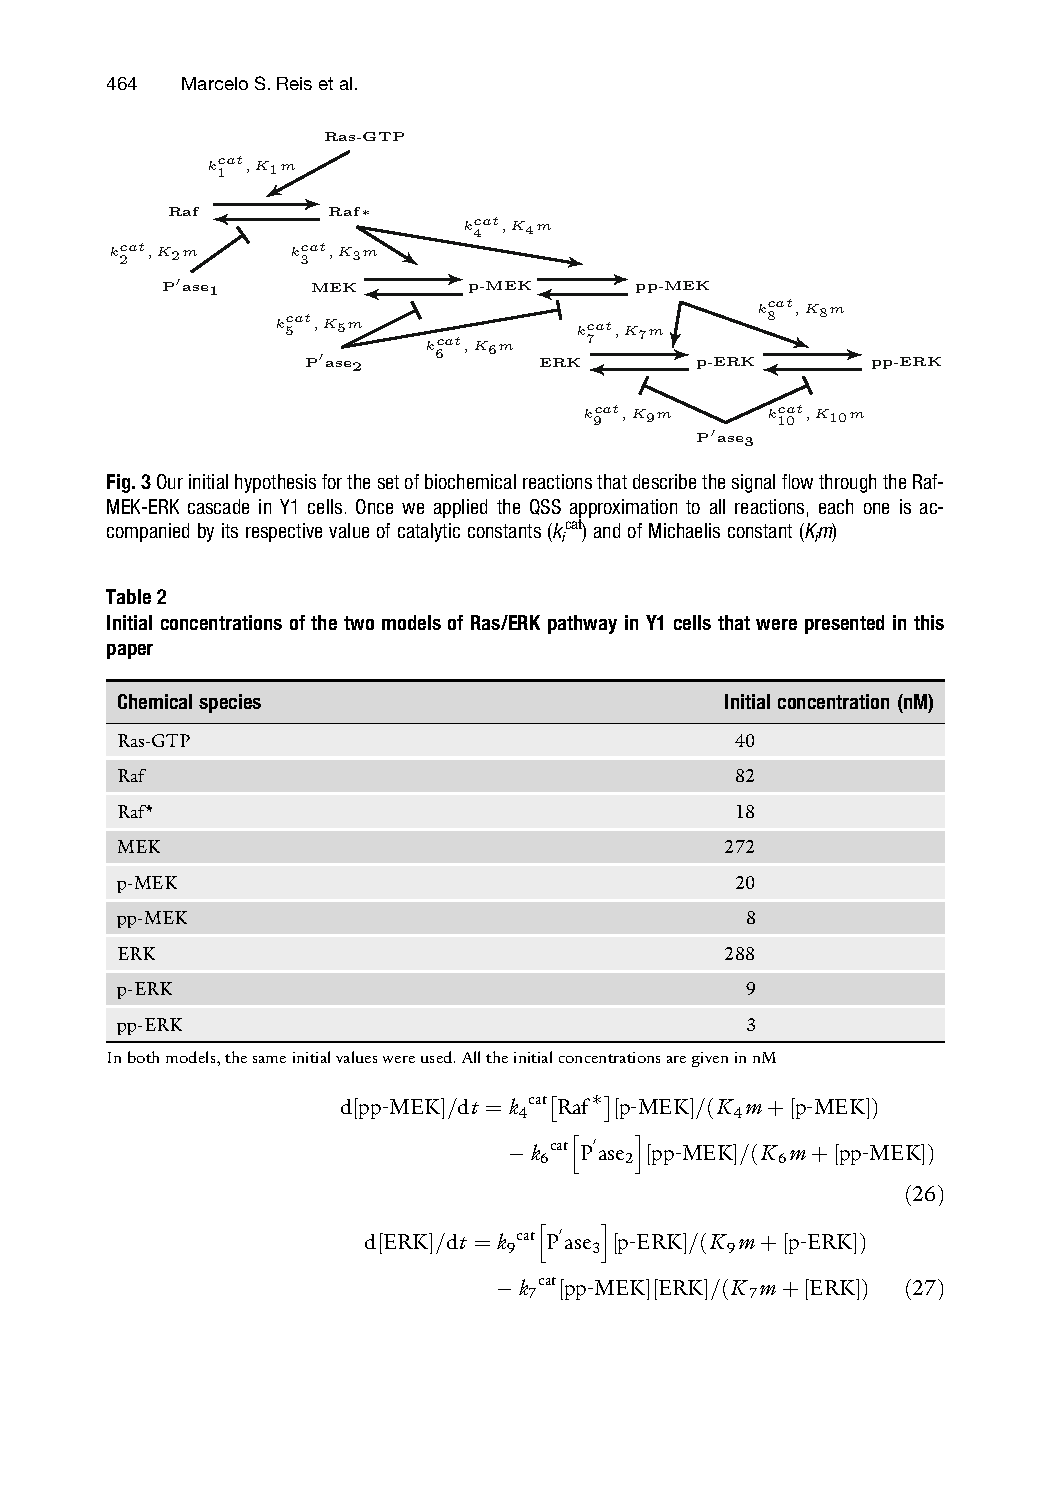
\includegraphics[width=\textwidth, viewport=40 500 460 660, clip]{introduction/signal_pathway_example_full_page.pdf}
\caption{The above diagram show a hypothesis for a signaling pathway 
    that flows through Raf-MEK-ERK cascade. Names in bold represent 
    chemical species. Names in italic represent parameters of the 
    ordinary differential equation of each interaction.Horizontal arrows
    represent phosphorylation when directed from left to right or 
    dephosphorilation when directed in the opposite direction. Other 
    arrows represent positive feedback if they are directed downwards or 
    negative feedback otherwise. Image copied from Marcelo S. Reis et.
    al (2017)~\cite{Reis2017}.}
\label{fig:signal_pathway_example}
\end{figure}

The first task one must complete to create a model is to determine a set 
of interactions to consider in the ODE system. Searching for pathway maps
on the Kyoto Encyclopedia of Genes and Genomes 
(KEGG)~\cite{Kanehisa2000kegg} is a good start. The KEGG PATHWAY 
Database provides manually drawn diagrams that represent signaling 
networks created with experimental evidences. However, it's possible 
that there's no pathway on KEGG that is able to correctly represent the 
biological experiment of interest; for those situations, it's necessary 
to modify the pathway by adding or even removing interactions. One might 
reason that we should use as many interactions as we can to get a better 
simulation, however, this usually implies in poor or computationally 
infeasible models because of two reasons: first, complex models will 
require more time in the numerical solution computation, which may be 
infeasible due to limited computational resources; and second, when 
considering many interactions, we are also placing many parameters 
(multiplying constants of the differential equations) on the model, and 
finding appropriate values for them becomes harder as we increase the 
number of parameters.

The second task to create a model is to find values for all the system
parameters. There are two approaches for this task, you can either 
fetch values for these constants from the literature or you can find 
values that makes the model output approximate the experimental 
observations. For the first approach, repositories such as 
BioModels~\cite{le2006biomodels} can be used; for the second approach, 
statistical and optimization methods can be used. For optimization, it 
is necessary to define a metric that can evaluate how close the 
parameters brings the model output to the experimental observation so
that you can search for the optimal parameter in the parameter space. 
Statistical inference, in the other hand, usually tries to maximize some 
likelihood function, which is defined to represent the probability of a 
model, with a set of parameter values, to reproduce the experimental 
observation.

% However, we might have missed some interactions or even added irrelevant ones
After completing both tasks, however, as we mentioned before, we might 
still not have found a model that fairly approximates the biological 
experiment of interest. That could indicate that the set of chemical 
interactions chosen for the model is incomplete or has interactions that
are not relevant for the biological experiment. Therefore, it is 
desirable to construct a systematic method of modifying the set of 
chemical reactions in order to find the optimal set.

% Lulu solved it as a combinatorial problem
With the title ``A method to modify molecular signaling networks through
examination of interactome databases"~\cite{Wu15} Lulu Wu presented in 
her masters dissertation a methodology to systematically modify 
computational models of signaling networks to better simulate biological 
experiments. Starting with a model that does not approximate well the 
biological data, this methodology proposes to add a set of interactions
to the model topology in order to better simulate the signaling pathway 
of interest. This set of interactions is a subset of interactions from a 
database created by Lulu Wu, joining information
from many static maps available on KEGG. The choice of this subset can 
be modeled as a combinatorial optimization problem in which the search 
space is the set of all possible subsets of interactions to be added.
The cost function of this problem, however, is not as simple to define 
as the search space. Note that the search space itself does not define 
models, but only the topology, i.e. the set of interactions, therefore, 
to consider the second task of creating computational models for 
signaling networks, the cost function must take into account the set of 
values for the model parameters. As an example, we could define the cost 
as the minimum distance between model and experimental measures 
considering all possibilities of parameter values; however, 
unfortunately, finding the minimizing parameter values is a hard 
problem.

Since this is a hard problem, the method presented by Lulu Wu 
implements a heuristic version of this cost function. This heuristics 
is based on a Simulated Annealing procedure that searches for a set of 
parameter values trying to minimize (as much as possible) the distance 
between model and experimental measures; the best found distance is then
considered as the cost of the model. Once the number of possible model 
topologies grows exponentially on the number of interactions from the 
database, the algorithm used to traverse the search space of subset of 
interactions is also a heuristic, and it is based on the greedy 
algorithm called Sequential Forward Selection (SFS)~\cite{Whitney1971}.
The heuristic implemented by Lulu Wu selects a fixed number of 
interactions from the database and then creates candidate models by 
adding to the current solution the respective interaction; then, after 
evaluating the cost function for each model, the algorithm moves to the 
best candidate.

%The work of Lulu Wu was succesful on 

% Her work however had a few flaws...
% To surmount these limitations
% - gather information from many data sources
% - create new search algorithms
% - use Bayesian approach 


\chapter{Fundamental concepts}
\label{chap:fundamental_concepts}
%begin-include

In this section we provide the concepts that are fundamental to 
understand the biological and computational problems, methodologies and
results that we will present in this work. We start this chapter 
presenting what is a cell signaling pathway and how can one take 
measures to identify its activity on the cell. Later we present how 
it is possible to represent chemical iteractions as differential 
equations, and how that allows one to model a cell signaling pathway
with a system of ordinary differential equations. Then, we present 
more formally the problem we are trying to solve on this project, the
identification of cell signaling pathways, as well as the state of the
art methods of model ranking. Finally, we present the basics of 
posterior distribution sampling, which is a useful tool when working 
with Bayesian approaches, such as the ones used on this project to rank 
models.

% What I want to talk about in this section?
% - Cells signaling pathways are part of the cell communication system,
% and it allows the cell to perceive the conditions of the environment 
% and also to change its behaviour according to the input signal.
% - The signals perceived by a cell can come from cells that very close
% (including itself), as in synapses or it can travel long distances in 
% the organism, as in hormones.
% - When a signal reaches a cell, it can either activate a receptor in
% the cell membrane or diffuse into the cell.
% - Once this happen, the signal or the activated receptor can trigger
% a sequence of chemical interaction, altering the conformation and 
% state of proteins and also changing the concentration of chemical 
% species in the cell. Ultimately, this chain of effects can alter the 
% behaviour of the cell, what is called signal transduction.
% - Studying signaling pathways is important because they help us 
% understand the mechanisms of a cell, which can for example, elucidate 
% treatments for diseases.
\section{Cell Signaling Pathways}
Cell signaling pathways are part of the complex cell communication 
system, and it allows the cell to perceive the conditions of the 
environment in which it is placed and change its behaviour accordingly.
Signaling pathways participate in the regulation of many cell functions,
including development, division and cell death~\cite{Hancock2017}. The
dynamic of a signaling pathway can also be releated to diseases, as in
many cases of cancer.

The signal perceived by a cell can come from cells that are close 
(including the same cell that produced the signal), as in synapses, or 
it can travel long distances in the organism, as in hormones. When a 
signal reaches a cell, it binds to a specific receptor in the membrane,
and once that happens, the receptor can trigger a sequence of chemical 
interactions that can include change of conformation of proteins, 
activation or inactivation of proteins, and change of concentration of
chemical species in the cell. Ultimately, this chain of chemical 
reactions caused by the signal can alter the behaviour of the cell, what 
is called signal transduction.

Since signaling pathways participate in many of the cell functions, and 
are also related to diseases, it is important to study those structures
in order to get a better understanding of the cell mechanisms and 
diseases. One approach on the study of the cell signaling pathways is to 
measure the concentration change of proteins and how they interact to
produce those changes.

% - Western blot is a technique that can indicate the amount of a 
% specific protein that is in a mixture of proteins
% - This technique shows the presence of a protein in a mixture by 
% ``blotting'' these molecules into a membrane. 
% - Repeating the procedure in different times define time-course 
% observations of the protein in a biological experiment.
% - With these observations in hand, the researcher is able to construct 
% a measurement that is relevant to describe the biological experiment. 
% For instance, in a signaling network where a protein is closely 
% related to the behaviour of interest of the cell, this protein is a 
% good candidate as a measure of the system.
\section{Measurements of Proteins in Cell Signaling Pathways}
Western blot~\cite{Towbin1979} is a laboratory technique that can 
indicate the amount of a specific protein that is present in a mixture. 
This technique shows the presence of a protein in a mixture by 
``blotting'' a membrane where the molecules of interest are located. We 
can summarize the procedure in the following steps: first a mixture 
containing a sample of cells of interest must be created; 
second, proteins from the mixture should be fixed on the blotting 
membrane; third, an antibody should bind to the target protein 
molecules; and finally, a method for highlighting the bound antibody 
should be applied. An image of the resulting membrane can then be 
analyzed with computer programs to quantify the relative concentration 
(with respect to some other protein, usually a control protein that has 
fairly the same concentration during the whole experiment) of the 
protein of interest.

By repeating this procedure in different times it is possible to create 
time-course observations of proteins throughout the biological 
experiment. With this tool, a researcher can choose a set of relevant 
proteins from a signaling network and gain knowledge about the dynamics 
of such chemical species during the experiment. For instance, in a 
signaling network experiment in which it is desired to understand how
the change of concentrations of a species at the beginning of the 
pathway changes the concentration of some species at the end of the 
cascade, then measurements of both are relevant to understand the 
biological experiment. Figure~\ref{fig:western_blot_example} presents an 
example of time-course Western blot for an experiment where it is 
desirable to understand how extracellular signal-regulated kinase (ERK)
is activated (phosphorylated) as a function of levels of Rat sarcoma
bound to guanosine triphosphate (Ras-GTP).

\begin{figure}[!ht]
\centering
    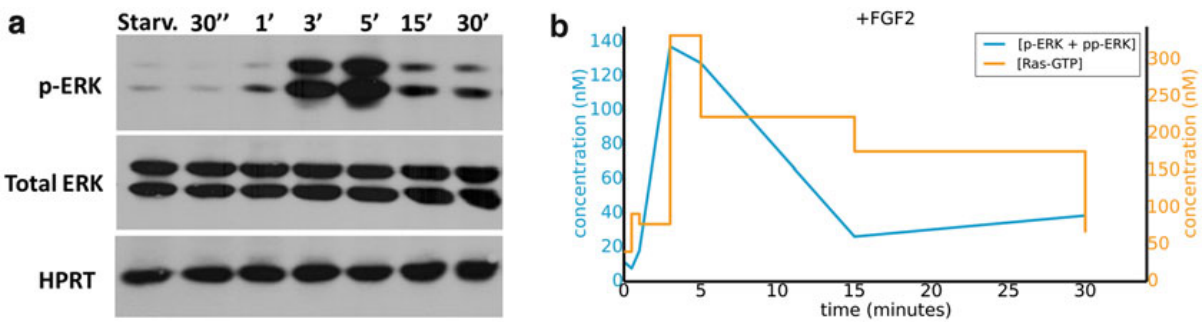
\includegraphics[width=\textwidth]{fundamental_concepts/western_blot.png}
    \caption{Figure {\bf a} shows time-course measurements of ERK, 
    phosphorylated ERK (p-ERK) and hypoxanthine-guanine 
    phosphoribosyltransferase (HPRT). HPRT is a ``loading'' protein, 
    that means that its concentration is fairly the same through the 
    experiment, and therefore it is used as a normalizing factor to 
    total ERK concentration. Figure  {\bf b} shows values of 
    phosphorylated ERK that are obtained after processing Figure 
    {\bf a}. Original image of Marcelo S. Reis et al. 
    (2017)~\cite{Reis2017}.}
    \label{fig:western_blot_example}
\end{figure}

These measurements alone do not always provide means for researchers to 
understand a cell signaling pathway experiment. However, if we create a 
computational model for this signaling networks that is able to 
reproduce experimental data, then we might use this model as a 
summary of the signaling network, which can provide to researchers 
evidences of the biological phenomena.


% What do I need to talk about?
% - We can model the concentration changes of chemical species as 
% differential equations, using the mass-action kinetic laws
% - The mass action kinetic law states that in an elementary reaction,
% the rate of a chemical reaction is directly proportional to the 
% product of the reactants concentrations.
% - What is elementary?
% 2.1 Elementary reactions rate equations
% - Types of elementary: first order reaction and second order reaction
% - How do we write up these two? 
% - Chemical notation with constants
% - From there we can write a system of differential equations to 
% describe the signaling pathway.
% - As an example, let's show the equations for a simple enzymatic 
% equation.
% 2.2 Simplifications of reactions
% - More can be done. We can simplify some equations 
% 2.1 Mass conservation simplification
% 2.2
\section{Dynamic Modeling of Cell Signaling Pathways}
One approach onto modeling cell signaling pathways is to model the 
dynamics of the concentrations of chemical species involved. This can be
accomplished when using the law of mass action~\cite{Voet2010}. This law 
states that, in an elementary reaction, the speed (or rate) of a 
chemical reaction is proportional to the product of the concentration of 
all reactants. An elementary reaction is a reaction in which there is no 
participation or need of an intermediate reaction to describe the first 
in a molecular level. In practice, it is more common to see two types of 
elementary reactions, they are first or second order reactions. 

\subsection{Modeling Elementary Reaction Rates}
A first order reaction is composed of one reactant only. Suppose A is 
the only reactant and B is the only product of a reaction, then we can
write this reaction as:
\begin{equation*}
\ce{
    A -> B
}.
\end{equation*}
The reaction rate of this reaction, according to the law of mass 
action, is 
\begin{equation*}
    k_1[\text{A}],
\end{equation*}
where $k_1$ is some constant and [A] is the concentration of A. It is
import to note that the constant $k_1$ is a rate coefficient of the 
reaction and, therefore, it can only assume positive values.

A second order reaction is composed of two reactants. Suppose C and D 
are both and the only reactants and F is the product of a reaction, then
we can write this reaction as:
\begin{equation*}
\ce{
    C + D -> F
}.
\end{equation*}
The reaction rate of this reaction is:
\begin{equation*}
    k_2\text{[C][D]},
\end{equation*}
where $k_2$ is a (positive) constant and [C] and [D] are the 
concentrations of C and D, respectively.

Using these two laws to calculate the speed of reactions, we are able 
to describe how the concentration of chemical species in a system change 
through time using differential equations. To illustrate this and future 
concepts of this section, we are going to consider a minimal system 
composed of a simple enzymatic reaction:
\begin{equation}
\ce{
    E + S <=>[\ce{$k$_f}][\ce{$k$_r}] ES ->[\ce{$k_{cat}$}] E + P
},
\label{eq:simple_enzymatic}
\end{equation}
where E is an enzyme, S is a substrate, ES is the enzyme-substrate
complex, and P is the product.

Each arrow in Equation~\ref{eq:simple_enzymatic} represents one 
elementary reaction, and the names over or under arrows represent 
reaction rate constants. All three reactions can be represented by the
equations:

%The first reaction has E and S as reactants and
%ES as a product, and can be written as 
\begin{subequations}
\begin{align}
\ce{
    E + S ->[\ce{$k_f$}] ES 
} \label{eq:es_complex_fwd} \\
\ce{
    ES ->[$k_r$] E + S
} \label{eq:es_complex_rev} \\
\ce{
    ES ->[$k_{cat}$] E + P
} \label{eq:es_pe} 
\end{align}
\end{subequations}
and they have, respectively, reaction rates of:
\begin{equation*}
\begin{aligned}
    & k_f\text{[E][S]} \\
    & k_r\text{[ES]} \\
    & k_{cat}\text{[ES]}.
\end{aligned}
\end{equation*}

Now, to determine a model of the concentration dynamics for
Reaction~\ref{eq:simple_enzymatic}, we will write a system of ordinary
differential equations. To do so, we should take every chemical species 
and calculate its concentration change rate based on the rate of each 
reaction that it participates. For instance, the enzyme E is a 
reactant on Reaction~\ref{eq:es_complex_fwd} and is also a product on 
reactions~\ref{eq:es_complex_rev} and~\ref{eq:es_pe}, then we consider 
that E changes its concentration over time ($t$) according to the 
differential equation:
\begin{equation}
    \frac{d[\text{E}]}{dt} = -k_f\text{[E][S]} + (k_r + k_{cat}) \text{[ES]}
\end{equation} 
Note that we are adding reation rates in which the species is a product
and we are subtracting reaction rates in which the species is a
reactant. Repeating this procedure for every other species of the 
enzymatic reaction leads to the following system of ordinary 
differential equations:
\begin{subequations}
    \label{eq:full_system}
    \begin{align}
        \frac{d[\text{E}]}{dt} & =  
            -k_f\text{[E][S]} + (k_r + k_{cat}) \text{[ES]} 
            \label{eq:dEdt} \\
        \frac{d[\text{S}]}{dt}  & = 
            -k_f\text{[E][S]} + k_r\text{[ES]} 
            \label{eq:dSdt} \\
        \frac{d[\text{ES}]}{dt} & =  
            k_f\text{[E][S]} - (k_r + k_{cat}) \text{[ES]} 
            \label{eq:dESdt} \\
        \frac{d[\text{P}]}{dt} & = k_{cat}\text{[ES]} \label{eq:dPdt}.
    \end{align}
\end{subequations}

% Ok, what do I really want to talk about here: Michaelis Menten 
% simplification of enzymtic reactions
% - Before anything, we should use mass conservation to produce the 
% d[ES]/dt equation.
% - Then we should mention the steady-state proposal of Michaelis Menten
%   -> should I use a picture? Maybe I can compare two initial states,
%      one with [S] >> [E] and the other not.
% - Mention that we can suppress a lot of parameters with this 
%   simplification
\subsection{Simplification of Dynamic Models}
The System~\ref{eq:full_system} can be simplified if we
apply properties of enzymatic reactions together with algebraic 
simplifications. We will show then how to derive the quasi-steady-state 
Michaelis-Menten model for enzymatic reactions. With the correct 
assumptions, this model is able to reproduce the behaviour of an 
enzymatic reaction without considering the intermediate enzyme-substrate 
complex.

A basic the principle we need to apply to our system in order to derive
the Michaelis-Menten model is the principle of mass conservation. This 
principle is valid if we assume that the 
reactions~\ref{eq:simple_enzymatic} are isolated, meaning that the 
chemicals on these reactions are not involved in other reactions at the
same time. Applying this principle to the enzyme chemical, produces the
following equation:
\begin{equation*}
    \text{[E$_0$]} = \text{[E] + [ES]}.
    \label{eq:E_conservation}
\end{equation*}
If we apply this equation to the derivative of the concentration of ES,
we will get the following equation:
\begin{equation}
    \frac{d[\text{ES}]}{dt} =  
        k_f(\text{[E$_0$]} - \text{[ES]})\text{[S]} 
        - (k_r + k_{cat}) \text{[ES]}. 
        \label{eq:dESdt_2}
\end{equation}

One more assumption is necessary to derive the simplification. This 
assumption states that the concentration of substrate-enzyme complex
does not change over time, i.e. $\frac{d[\text{ES}]}{dt} = 0$, and it 
was first proposed in 1925 by Briggs and Haldane~\cite{Briggs1925}. 
Generally, this assumption is applicable whenever [S] $\gg$ [E]. 
Applying this assumption together with the mass conservation assumption 
on the Equation~\ref{eq:dESdt_2}, we get:
\begin{equation*}  
    \begin{aligned}
        \text{[ES]} (k_r + k_{cat}) &= 
            k_f(\text{[E$_0$]} - \text{[ES]})\text{[S]}, \\
        \text{[ES]} &= \frac{\text{[E]}_0\text{[S]}}{K_m + \text{[S]}}, 
    \end{aligned}
\end{equation*}
in which $K_m = \frac{k_{cat} + k_r}{k_f}$ is known as Michaelis 
constant. Considering this, we can rewrite the rate of [P] as:
\begin{equation}
    \frac{d\text{[P]}}{dt} = k_{cat}\frac{\text{[E]}_0\text{[S]}}
        {K_m + \text{[S]}}.
    \label{eq:dPdt_2}
\end{equation}
And finally, if we apply mass conservation to the substrate, we will get
the following equation:
\begin{equation*}
    \text{[S$_0$]} = \text{[S] + [ES] + [P]},
\end{equation*}
then, we can differentiate this equation on $t$ and use the 
quasi-steady-state assumption ($\frac{d\text{[ES]}}{dt} = 0$) to obtain:
\begin{equation}
    \frac{d\text{[S]}}{dt} = - \frac{d\text{[P]}}{dt}.
    \label{eq:dSdt_2}
\end{equation}

Now, with equations~\ref{eq:dPdt_2}~and~\ref{eq:dSdt_2} we are able to
reproduce the dynamics of the substrate and product of the enzymatic 
reaction. Therefore, using the Michaelis-Menten model, we could simplify 
the System\ref{eq:full_system} that had four equations and three 
parameters to a new model that has only two equation and two parameters 
($k_{cat}$ and $K_m$). Figure~\ref{fig:michaelis_menten} shows a 
comparison between the complete and Michaelis-Menten models of enzymatic 
reactions.

\begin{figure}[H]
  \centering 
  \begin{tabular}{c c}
    \subfigure[] {\scalebox{1}{
    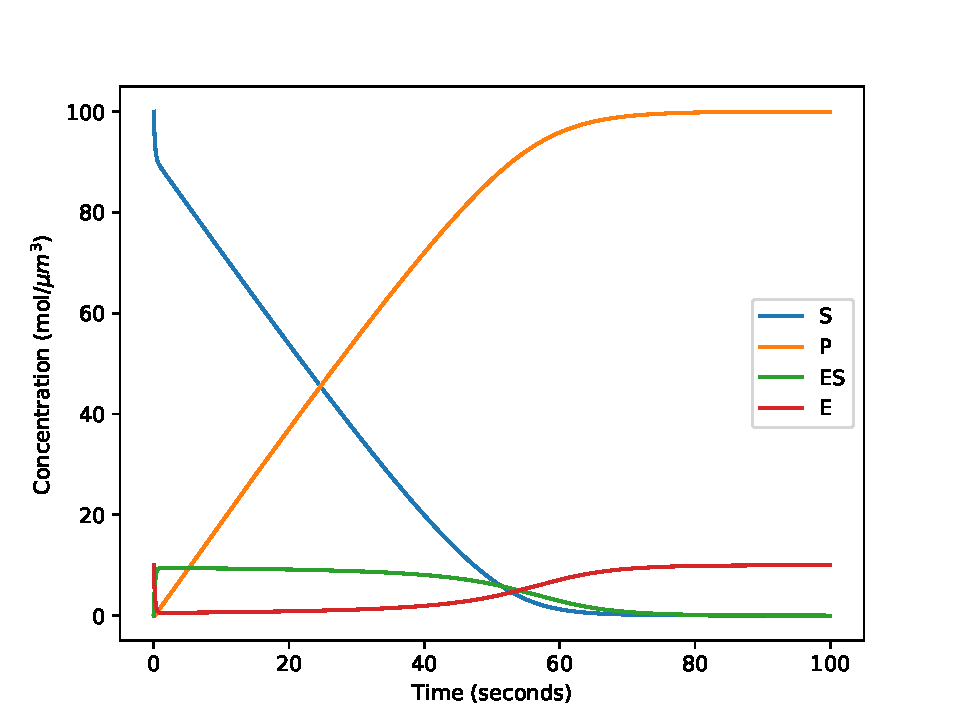
\includegraphics[trim={0 0 0 1.4cm}, clip=true, width=.45\textwidth]{fundamental_concepts/simplifications/full_system.pdf}}
     \label{fig:enzymatic_full}}
     &
    \subfigure[] {\scalebox{1}{
    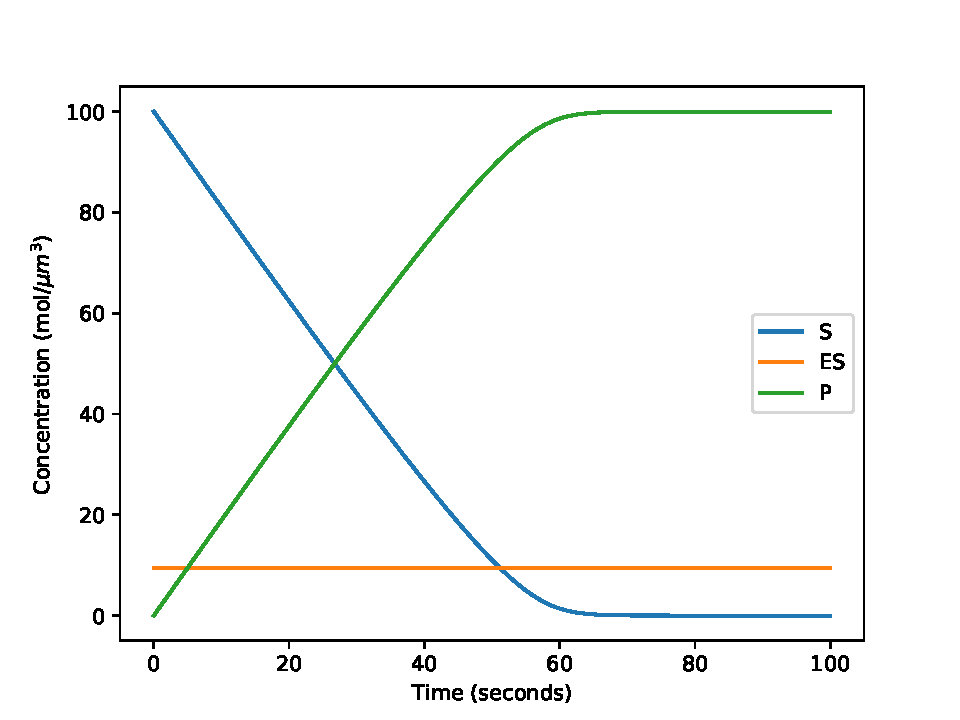
\includegraphics[trim={0 0 0 1.4cm}, clip=true, width=.45\textwidth]{fundamental_concepts/simplifications/mm_system.pdf}}
    \label{fig:enzymatic_mm}}
  \end{tabular}
    \caption{An example of the dynamics produced by two models of 
        enzymatic reactions. The Figure~\ref{fig:enzymatic_full} 
        presents the dynamics of the model~\ref{eq:full_system} and 
        Figure~\ref{fig:enzymatic_mm} presents the dynamics of the 
        Michaelis-Menten simplification to the same model. For this 
        simulations, it is necessary to define initial concentrations of
        the chemical species involved, and it is used: 
        10 molecules$/(\mu m)^3$ for the enzyme (E); 
        100~molecules$/(\mu m)^3$ is used for the substrate (S); and 
        0~molecules$/(\mu m)^3$ is used for the other species. In 
        addition to this, it is also necessary to define model 
        parameter values, and it is used: 
        0.06~$(\mu m)^3$(molecules$*s)^{-1}$ for $k_f$; 
        0.1~$(s^{-1})$ for $k_r$; 0.2~($s^{-1}$) for $k_{cat}$; and,
        following the Michalis-Menten model, 5 molecules$/(\mu m)^3$
        is used for $K_m$.}
  \label{fig:michaelis_menten} 
\end{figure}

% What to talk about:
% 1. Define identification of cell signaling pathways
%    -> Identification of signaling pathways is the problem of finding 
%       the components of a signaling network and how they interact 
%       in order to reproduce some behaviour of the cell that was
%       previously measured experimentally. 
%    -> The input of the problem should be then a description of the 
%       biological experiment and the measurements made on this 
%       experiment. As an output, we are expected to give a topology
%       of the network of interactions that are actively controlling
%       the cell behaviour observed on experiment measurements. More 
%       than that, we are also supposed to determine the set of 
%       parameter values that should be used on the models to reproduce
%       measurements similar to the experiments (or a probability 
%       distribution).
%    -> Two main tasks onto creating the output: you have to find 
%       a topology that is good with some parameter to reproduce the 
%       experiment; note that these tasks are very strongly correlated
%       and should be done together. 
% 2. Explain the challenges of cell signaling pathways
%    -> Firstly, simulating these problems is very time-consuming (even 
%       tough there are many ode solvers out there)
%    -> The number of possible interactions is very big. If we consider
%       choosing from n interactions a subset of them that should be on 
%       the topology, then there are 2^n options.
%    -> Once you choose two candidates of topology, it is still hard to
%       tell which one is better.
% (?). Talk about the work of Marcelo. State that current solutions do
%       not systematically search for the solution. 
% 3. somehow link to the next section, about cost functions 
%    -> Many of the state of the art approaches on identification of 
%       cell signaling network are based on a Bayesian approach for 
%       model ranking.
\section{Identification of Cell Signaling Pathways}
Identification of signaling pathways is the problem of finding the 
components of a signaling pathway and how they interact in order to
reproduce a behaviour of the cell that has been previously measured 
experimentally. The input of this problem is usually a description of 
the biological experiment, containing previous information about the 
signaling pathway, and a set of measurements, commonly Western blot 
data. The output to this problem is then composed of a set of 
interactions that are actively controlling the behaviour of interest of 
the cell, and also the set of parameter values that should be used on 
these interactions to create a model that approximates the experimental 
observations; it is possible to output a single value for each 
parameter, as it was presented in~\cite{Wu15}, or output information 
about these values, using a posterior (to the experimental data) 
distribution, as it was presented in~\cite{Liepe2014}~and~\cite{Xura20}.

Two main tasks must be completed to produce this output. The first task
is to find candidate topologies for the pathway model, i.e. different
set of interactions that are relevant to the pathway of interest. The
second task is to rank those models according to their ability to 
simulate the pathway and approximate the experimental measurements.

% To the second task, you can use combinatorics optimization to fit the
% model to the data and calculate the distance of the measurements on 
% the fitted model to the experimental data; then it is possible to rank
% models according to this distance. Alternatively, it is 
% possible to consider that the model parameters are random variables 
% and calculate the marginal probability of the model to reproduce the 
% observed data; then, it is possible to rank models according to this 
% probability.

The second task is also known as the model selection problem and even
though it is a broad area, there are works on the literature that treats 
specifically the problem in a biochemical context. Solutions to this 
problem should be able to choose model candidates according to their 
ability to reproduce observed data and penalize overly complex models 
to avoid overfitting. 

One approach on setting the score of a model is to search for the set of 
parameter values that makes the model measurements the closest to the 
experimental data and then define a distance between these two 
measurements; then it is possible to use this distance plus a penalty 
for complexity to create a ranking of the models. We can write this 
scoring function as:
\begin{equation*}
    score_1 (M) = - min_{\{\theta \in \Theta' \subset \Theta\}}  
        dist (\phi(M, \theta), D) + R (M),
\end{equation*}
where $M$ is the model, $\Theta$ is the parameter space, $\Theta'$ is 
the subset of the parameter space where the search for the best 
parameter values was conduced, $D$ is the experimental measurement,
$\phi$ is a function that determines the simulated measurement on the 
model, and $R$ is a regularization function that penalizes model 
complexity. This approach was implemented on the work of Lulu 
Wu~\cite{Wu15}, using a Simulated Annealing procedure to search for 
parameter values that minimizes the distance between simulation and 
experiment. The Simulated Annealing procedure used is available on the 
software SigNetSim (Signaling Network Simulator), which is based on the
of the work of Chu on~\cite{Chu1999}. However, Wu's methodology showed 
limitations when testing the ability to reconstruct models from 
experiments, and this could be related to the used penalization term. 
In fact, choosing a good regularization function is crucial to the 
performance of this methodology.

Another approach is to consider the model parameters as random variables 
and then marginalize the probability of the model and parameters to 
reproduce the observed data, i.e. estimate (because calculating is 
usually hard) the marginal probability:
\begin{equation}
    p (D | M) = \int_{\Theta} p (D | M, \theta) p (\theta | M) d\theta,
    \label{eq:marginal_likelihood_integral}
\end{equation}
where $D$ is the observed data, $M$ is the model and $\Theta$ is the 
parameter space. The function $p(\theta | M)$ is the prior probability 
function of the parameter $\theta$ on model $M$ and the function 
$p (D | M, \theta)$ is the likelihood of observing the data $D$ when
simulating the model $M$ using parameters $\theta$. Sometimes, however,
the likelihood function is unknown or computationally intractable; for
these cases, it is possible to use an alternative Bayesian approach, 
called Aproximate Bayesian Computation (ABC), to estimate the 
probability $p (M | D)$ and use it as a ranking score~\cite{Toni2009}.

% However, to the first task, there are not many methods on the 
% literature to solve this problem. Generally, this is solved using 
% both interactome maps from KEGG and the prior knowledge of the 
% researchers.
For the first task of identification of signaling pathways we described, 
the creation of model candidates, there are not as many works on the 
literature as there are for the second task. Commonly, researchers must 
resort on their own knowledge on the biological experiment and consult 
interactome maps available on repositories such as KEGG and BioModels to
construct manually the hypothesis of models for a signaling pathway. 
That enlightens the importance to create a methodology that 
systematically creates candidate models of signaling networks, as we 
propose on this project.



% What are the best approaches on model selection recently
% -> Most of them uses Bayesian ideas
% -> good because they can provide statistical formality about the 
%    selection.
% -> automatic penalization; allows researcher to introduce biological
%    information through the priors.
% -> it makes sense that a parameter is a random variable
% -> Explain BIBm
% -> Explain ABC-SysBio
% -> Even though they provide ways of ranking models, they don't treat
% the modeling of the network topology.
% -> Bayesian approaches
\section{State of the Art in Selection of Biochemical Models}
The state of the art in biochemical model selection is based on Bayesian
inference. The Bayesian approaches provide the benefits of ranking 
models with statistical formalism, and automatically penalizes overly 
complex models. More than that, through the prior distribution of the
parameters, the researcher is able to input prior knowledge about 
interactions constants; this type of information can facilitate the 
parameter inference of models since it tends to concentrate the search.

Bayesian approaches consider that model parameters are random variables, 
instead of fixed unknown constants. We can argue that this modeling is 
fair to the reality in biochemical processes because interactions 
constants can vary depending on the cell conditions. Therefore, in a 
biological experiment in which there might be perturbations to the cell 
environment, it should be more adequate to rank models integrating the 
models score over a probability space of parameters instead of fitting 
the model to data using a single point of the parameter space. We will 
now present the basic concept of two methods that use this idea for 
model selection, the Annealing-Melting Integration 
(AMI)~\cite{Vyshemirsky2007} and Approximate Bayesian Computation 
(ABC)~\cite{Toni2009}.

% What to mention about AMI:
% -> thermodynamic integral
% -> we are estimating the log of p(D|M, theta)
% -> theta being distributed according to some q_beta (\theta)
% -> q_beta are bridging distributions from prior to posterior
% -> to estimate this integral we need to use Monte Carlo Markov Chains
The Annealing-Melting Integration is a method that estimates the 
integral~\ref{eq:marginal_likelihood_integral} using concepts of 
thermodynamics. With thermodynamic integration, it is possible to write 
the logarithm of this integral as:
\begin{equation}
        \ln p(D|M) 
            = \int_0^1 \expectation_{q_\beta(\theta)} 
              [\ln p(D | M, \theta)] d\beta
        \label{eq:thermodynamic_integral}
\end{equation}
where $p(D|M,\theta)$ is the likelihood function (the 
probability of observing the data D when $M$ is the correct model, with
parameters $\theta$); and $\expectation_{q_\beta (\theta)}$ is an 
expectation taken over the probability space of $q_\beta(\theta) 
\propto p(D|M, \theta)^\beta p(\theta|M)$. The 
variable $\beta$ works in the integral as a temperature term, 
determining the probability functions $q_{\beta}(\theta)$; note that 
when $\beta = 0$ then 
\begin{equation*}
q_0(\theta) = p(\theta|M),
\end{equation*}
the prior distribution of the parameters, and when 
$\beta = 1$ then 
\begin{equation*}
    q_1(\theta) = \frac{p(D, \theta| M)} {\int_{\Theta}
                            p(D, \theta| M)} 
                = \frac{p(\theta | D, M)p(D|M)} 
                        {p(D | M)}
                = p(\theta | D, M),
\end{equation*}
the posterior distribution of parameters. Therefore, the 
integral~\ref{eq:thermodynamic_integral} takes the expected value of the
likelihood function of $D$ over a sequence of probability distributions
that is a ``bridge of distributions'' connecting the prior and posterior 
distributions of parameters. Calculating the integral is usually 
infeasible, hence in practice it is needed to estimate this integral 
using samples of a finite number of tempered distributions, 
$q_\beta(\theta)$.

% How about ABC?
% -> Likelihood free!
% -> Define the algorithm
%   -> The goal of the algorithm is to find a ``good" sample of 
%      parameters for the observed data.
%   -> The algorithm proposes a candidate parameter \theta*.
%   -> Simulate the model with those parameters.
%   -> Using a distance function d, accept theta* if
%      d(simulation, data) < eps
As we mentioned before, the likelihood function 
$p(D | M, \theta)$ may be very hard to calculate if not 
impossible. For those cases it is possible to use parameter inference
approaches that are likelihood-free, called Approximate Bayesian 
Computation (ABC). This method has the goal of producing a sample of 
parameters that brings the model simulations close to the observed data.
A generic ABC algorithm starts proposing a candidate parameter 
$\theta^*$ from a proposal distribution; then, a simulation, 
$\phi (M, \theta^*)$ of the model using the candidate parameters is 
produced; if, for some distance function $d$, is true that 
$d(\phi(M, \theta^*), D) < \epsilon$, then we accept $\theta^*$ as part
of the sample. If $\epsilon$ is sufficiently small, then the produced
samples approximates well the posterior distribution. To use ABC methods
for model selection it is enough to add a model indicator parameter to 
the parameter array, then it is possible to extract model distribution
of the accepted parameters.

% Metropolis-Hastings algorithm
% -> Both methods for model selection, based on ABC or using 
% thermodynamics integration needs to generate samples of probability 
% distributions. Generating samples of distributions is easy for many 
% well known distributions, however, for some other distributions it may
% not simple. 
% -> What does it do?
% Metropolis-Hastings algorithms are capable of generating a
% sample that has some probability distribution $p$, the target 
% function. The method can be used even when it is not possible to 
% calculate points of the target probability function, because all it is
% needed is a function that is proportional to the target. This is 
% useful for example when the target function is a posterior
% -> How do we do this
%   -> 
\section{Metropolis-Hastings to Generate Samples}
Both methods for model selection, based on ABC or using thermodynamics
integration need to generate samples of probability distributions. 
Generating samples of distributions is simple for many well known 
distributions, however, for some other distributions it may not be as
simple. Metropolis-Hastings algorithms are capable of generating a 
sample that has some probability distribution $p$, which is called the 
target distribution. In fact, the method can be used even when it is not
possible to access directly the target function, because all it is 
needed to perform the sampling is a function that is proportional to the
target.

Being able to generate a sample of a target distribution without 
accessing the probability function itself is useful for our applications
in Bayesian model ranking. Consider that we need to create a sample of
the parameters posterior distribution $p (\theta | M, D)$. Calculating 
this probability function is very hard because
\begin{equation*}
    p(\theta | M, D) = \frac{p (D | \theta, M) p (\theta | M)}
                            {p (D|M)},
\end{equation*}
and this equation has the term $p (D|M)$, which is only known (by some 
estimation) at the end of the model ranking; however, if we can access
the likelihood function $p (D| \theta, M)$ and the prior 
$p (\theta | M)$ than the product of these two is proportional to the 
posterior distribution (since $p (D|M)$ is only a constant because it
does not depend on $\theta$), and therefore they are enough to generate
a sample of the posterior.

A generic Metropolis-Hastings algorithm that creates a sample of a 
target distribution $p (\lambda)$ proceeds as follows:
\begin{enumerate}
\item{Choose some starting point $\lambda_0$ for which $p (\lambda_0)$ 
    is not zero. Also set $t = 1$.}
\item{Sample a candidate point $\lambda^*$ from a proposal (or jumping) 
    distribution with probability $J_t (\lambda^* | \lambda^{t - 1})$.}
    \label{enum:iteration_start}
\item{Calculate the ratio:}
    \begin{equation}
        r = \frac{p (\lambda^*) J_t (\lambda^{t - 1} | \lambda^*)}
                 {p (\lambda^{t - 1}) J_t (\lambda^* | \lambda^{t - 1})}
        \label{eq:mh_ratio}
    \end{equation}
\item{With probability $min (1, r)$ set $\theta^t = \theta^*$ and set
    $\theta^t = \theta^{t - 1}$ otherwise.}
\item{Increase $t$ by one and, if not reached limit number of 
    iterations, go back to step~\ref{enum:iteration_start}.}
\end{enumerate}
Note that if the target $p (\lambda)$ is not available, and rather 
another function $q (\lambda) = \frac{1}{c}p(\lambda)$ is available, 
then the ratio~\ref{eq:mh_ratio} can be calculated as:
\begin{equation*}
    r = \frac{p (\lambda^*) J_t (\lambda^{t - 1} | \lambda^*)}
              {p (\lambda^{t - 1}) J_t (\lambda^* | \lambda^{t - 1})} 
      = \frac{(q (\lambda^*)c) J_t (\lambda^{t - 1} | \lambda^*)}
           {(q (\lambda^{t - 1})c) J_t (\lambda^* | \lambda^{t - 1})} 
      = \frac{q (\lambda^*) J_t (\lambda^{t - 1} | \lambda^*)}
              {q (\lambda^{t - 1}) J_t (\lambda^* | \lambda^{t - 1})}
\end{equation*}
More than that, if the proposal distribution is symmetric, the produced 
algorithm is called Metropolis algorithm and has the ratio 
$r = {p (\lambda^*)}/{p (\lambda^{t - 1})}$. 

Different implementations of the Metropolis-Hastings algorithm are 
possible. The possible changes include the choice of starting point,
the choice of proposal distributions and number of iterations. As an
example, some algorithms are adaptive in the sense that they can change 
the proposal distribution according to the acceptance rate of proposed 
points~\cite{Gelman2013}.


\chapter{Model selection methods}
\label{chap:model_selection}
%begin-include
{\color{blue} Simple description of the content of this chapter}.

\section{Model ranking using Marginal Likelihood}
% Simple explanation of this model ranking
% Describe the likelihood function 
% However, this is very hard to calculate
% It is possible to apply an Importance Sampling Estimator {cite 
% Newton and Raftery}. However, it was showed on {cite girolami again}
% that these methods do not perform well.
% Then it was proposed to use Thermodynamic Integration. Make it clear 
% that this allows us to create some estimators.
% Subsection - Thermodynamic Integration
% -> explain how to derive it
%   -> name what is the power posterior
% -> include here: how to estimate it?
% Subsection - Estimation of the Marginal Likelihood 
% -> We need to find samples of the posteriors
% -> Explain that we use the methodology of Xuan
% -> We use three Metropolis-Hastings
% -> A first burn-in step with jumps independent for each single 
% parameter. Adaptive Metropolis Hastings
% -> A second using a Variance-Covariance Matrix
% -> A third using populational MCMC
The marginal likelihood of an experiment measurement $D$ being 
reproduced by a model $M$, $p (D | M)$, can be used as a model ranking 
metric as it determines which model makes the experimental observations 
more likely to happen. Before defining how to calculate the  marginal 
the likelihood, we must define what the likelihood function is. To 
calculate the likelihood $p (D | M, \theta)$, we must understand that 
conditioning the observation to the model and parameters means that in 
the probability space from which $D$ is taken, the model $M$ is the 
``real'' model and it has the parameter values of $\theta$; i.e. the 
model $M$ with parameters $\theta$ controls the behaviour of the system 
from which $D$ was observed. Then, assuming that the observations have a 
Gaussian error, and that they are taken in a time series of $m$ time 
steps, we can define the likelihood as:
\begin{equation}
    p (D | M, \theta) = p_{\mathcal{N}_{\left(\vec{0}, \Sigma\right)}}
        (\phi (M,\theta) - D),
\label{eq:likelihood_multivariate}
\end{equation}
where $\phi (M, \theta) \in \fieldR^m$ is the experimental measurement 
on the simulation generated by the model $M$ with parameters $\theta$,
and \smash{$p_{\mathcal{N}_{(\vec{0}, \Sigma)}} (\cdot)$} is the 
probability density function of a Multivariate Normal variable with mean 
$\vec{0}$ and covariance matrix $\Sigma$. As a matter of fact, as it is
done in the work of Xu et al., we can consider that the observation 
error is independent for each time step~\cite{Xura20}, therefore we can 
simplify~\ref{eq:likelihood_multivariate} to:
\begin{equation}
    p (D | M, \theta) = \prod_{i = 1}^m p_{\mathcal{N}_{\left(0, 
        \sigma^2\right)}} (\phi_i (M,\theta) - D_i).
\label{eq:likelihood}
\end{equation}
The $\sigma^2$ used in equation~\ref{eq:likelihood} is also a parameter
of the model, which means that, for some $k$, $\theta_k = \sigma^2$.

Now that we defined the likelihood function, we can write the marginal 
likelihood as:
\begin{equation}
    p (D | M) = \int_{\Theta} p (D | M, \theta) p (\theta | M)d\theta.
\label{eq:marginal_likelihood}
\end{equation}
However, calculating this integral analytically is only possible in 
very special cases and, usually, it would depend on knowing models for 
the distributions associated to these probability functions, which is 
generally not possible in our case.

Even though this integral is very hard to be calculated, there are 
methods that allow us to estimate its value. A straight forward method 
to estimate this integral value is the Importance Sampling 
Estimator~\cite{Newton1993}. This method uses the Monte Carlo integral 
estimation method that can estimate integrals of the form 
$\int g(\lambda) p(\lambda)d\lambda$ using the estimator:
\begin{equation}
    \hat{I} = \sum_{i = 1}^m w_i g(\lambda_i) / \sum_{i = 1}^m w_i,
\label{eq:importance_sampling_estimator}
\end{equation}
where $w_i = p (\lambda) / p^* (\lambda)$, and $p^*(\cdot)$ is known as 
the importance sampling function. If we set $\lambda = \theta | M$ and
use the prior ($p(\theta | M)$) or the posterior ($p(\theta | M, D)$) as 
importance sampling functions, then we would get respectively the 
estimators:
\begin{equation}
\begin{aligned}
    \frac{1}{m} \sum_{i = 1}^m p(D|M, \theta^{(i)}) &&& 
        (\text{with } \theta^{(i)} \sim p(\theta|M)); \\
    \left(\frac{1}{m} \sum_{i = 1}^m p(D|M, \theta^{(i)})^{-1} \right)^{-1} &&&
        (\text{with } \theta^{(i)} \sim p(\theta|M)).
\end{aligned}
\end{equation}
However, as showed by Vyshemirsky et al. (2007), these estimators might
produce very large variances and may not perform well for biochemical
model selection applications. For that reason we decide to use a 
Annealing-Melting method as it is proposed in the same 
work~\cite{Vyshemirsky2007}.

% ABC-SysBio
% Experiments comparing both approaches


\chapter{Development of SigNetMS, a software for model selection}
\label{chap:development_signetms}
%begin-include
In this chapter we present the development process and implementation
details of the SigNetMS software, which stands for {\bf Sig}naling 
{\bf Net}work {\bf M}odel {\bf S}election. This software is capable of
producing an estimative of the marginal likelihood of a model given
experimental data, $p({\bm D} | M)$.

% What are we going to talk about in this chapter?
% - first, we have to talk about which methodology this software uses
%   -> make sure you citate BioBayes and how its cumbersome to use it
% to create a model ranking. we should state that we are using marginal
% likelihood estimates here.
%   -> make sure we specify the input and output of this software
%   -> include program arguments
% - then, we can talk about the implementation and optimizations
%   -> how did we implement the sampling? what was the used proposal
%   distribution?
%   -> fast integration of system of differential equations
%   -> parallel sampling
%   -> running the algorithm on a cluster

\section{The SigNetMS Software}
% General Aspects of the software

% The Bayesian methodology
% - SigNeMS creates an estimative of the marginal likelihood of a model
% given a set of experimental data.
% - To create this estimative, SigNetMS uses ideas of Thermodynamic
%   Integration.
% - There is a software that can carry similar simulations, called
%   BioBayes, however we found its use cumbersome, mainly because:
%   it is a GUI software, which does not fit our type of applications,
%   that should be ran in a server for several hours. Moreover, we
%   intended to link the marginal likelihood output to other programs,
%   for model selection.

% Details on how the program creates the system of ODEs
% Details on how the proram estimates the likelihood

SigNetMS is a Python program that can be used as a tool for model
selection. The source code is available on 
Github\footnote{https://github.com/gustavoem/SigNetMS} and it is open
source, under the GNU General Public License.

This program expects as the input: a signaling pathway model,
represented by a Systems Biology Markup Language
(SBML)~\cite{hucka2003systems} file, with the definition of reactions,
kinetic laws and initial concentrations of chemical species; an
Extensible Markup Language (XML) file with experimental data, including 
time series measurements of the  biological phenomena of interest;
another XML file with definitions of prior distributions of reaction
rate constants; and, finally, a set of parameter values that determine
the sampling process of model parameters. There are also optional
parameters on SigNetMS, used to control random number generator seeds,
number of execution threads, and verbose runs.

The output of the program is composed by an estimative of the marginal
likelihood of the model, given experimental data, $p({\bm D} | M)$ and a
list of parameter values $({\bm \theta}^1, {\bm \theta}^2, \ldots {\bm
\theta}^l)$ that represent a sample of the distribution $p({\bm \theta}
| M, {\bm D})$. If one simulates the model $M$ with parameter values
from the sample, we expect that, the higher the marginal likelihood, the
closer the simulation is to the experimental data.

To calculate this estimative, we use the ideas of Thermodynamic
Integration we presented on section~\ref{sec:thermodynamic_integration}.
Before implementing SigNetMS we also considered using another software,
called BioBayes~\cite{Vyshemirsky2008}, that has a very similar approach
to produce an estimative of the marginal likelihood. However, we did not
proceed to use this software because there was only a graphical user
interface version of the software, which made the process of running
instances and collecting results cumbersome. We have also tried
contacting the authors to obtain the source code, however they could not
provide us that.

\section{Creating an estimative of the marginal likelihood}
% Since we are using a Thermodynamic Integration  approach, we need to 
% define a likelihood function, create samples of power posterior 
% distributions and, finally define an approximation to the marginal
% likelihood.

% The likelihood function...
% The samples of power posteriors are...
% The approximation of the marginal likelihood are...
% The whole process, has the following order:
% -> all inputs are read;
%   -> The sbml model is read and transformed into a System of ODE
%       -> this model can determine a simulation, given a list of
%       parameter values and a measurement unit;
%   -> Parameter priors, experimental data are read and saved
% -> sampling of posterior starts with naive sampling
% -> then we proceed to covariance shaped burn-in
% -> then we go to populational monte carlo markov chain
% -> then we use the approximation to generate the margginal likelihood

To create estimates of the marginal likelihood using the Thermodynamic
Integration approach, we need to define a likelihood function $p({\bm
D}| M, {\bm \theta})$ and also samples power posterior distributions
$p_\beta({\bm \theta})$ for a sequence of values of $\beta$. On
SigNetMS, we use the trapezoidal rule to approximate the marginal
likelihood, given by the
equation~\ref{eq:marginal_likelihood_trapezoidal_approximation}. 
Inspired by the work of Friel et al., we discretize the
interval $[0, 1]$ of power posteriors using the $\beta_i =
\left(\frac{i - 1}{T - 1}\right)^c$, where $T = 20$, $c = 4$ and $i \in
\{1, 2, \ldots, T\}$.

% TODO: say here that we used pipipi popopo beta values and that with
% samples of those power posteriors, we estimated the marginal
% likelihood as...

\subsection{Implementing the likelilhood function}
%-> The likelihood function is...
%-> To implement this, we must simulate the model with parameter values
%of theta.
%-> these simulations involves the numerical integration of a system of 
% ordinary differential equaitons
%-> current methods of numerical integrations are iterative and can be
% very consty depending on the size of the numerical system and also on
% the type of the system, stiff or not
The likelihood function we used is the same as we defined in
equation~\ref{eq:likelihood_multivariate}:
\begin{equation*}
    p ({\bm D} | M,{\bm \theta}) = 
        p_{\mathcal{N}_{\left(\vec{0}, \Sigma\right)}}
        (\phi (M, {\bm\theta}) - {\bm D}),
\end{equation*}
where ${\bm D}$ is the experimental measurement, $M$ is the model,
${\bm \theta}$ is a set of parameter values, $\Sigma$ is the variance of
the error of experimental observations, and, finally, $\phi$ is a 
function that calculates an approximation of the results of the
experiment that produced ${\bm D}$, applied to the simulated environment
of model $M$ with parameter values ${\bm \theta}$. This simulation of
the model is created by deriving a system of ordinary differential
equations, and then numerically integrating this system, over the time
steps defined by the experimental measurements. To reproduce the same
experiment that generated ${\bm D}$, SigNetMS expects that the XML file 
containing experimental data also contains a mathematical representation
of which quantity was measured, in terms of concentrations of chemical
species of the system.

% Numerical integration of systems are solved using iterative methods
% stiff non stiff
% we used  third-party software to solve this problem
The numerical integration of the system is alone a hard problem, and
therefore, we used third-party software to produce such integrations.
The most popular software available for this problem conduce
iterative algorithms that, step by step, approximate the state of the
system for a time interval. It is important to know that some instances
of the problem can be stiff, meaning that they may make the integration
algorithm be unstable, since it may need consecutive iterations in 
really small steps. Since we did not have time to go in details of when 
such cases occur, we chose third-party software that can adapt the used
algorithm according to the stiffnes of the instance.

After the implementation of the function $\phi$, most of the work to
implement the likelihood function is done. The remaining work is to
calculate the value of the probability density function
$p_{\mathcal{N}_{\left(\vec{0}, \Sigma\right)}}$ and that can easily be
accomplished using statistical packages such as
SciPy~\cite{2020SciPy-NMeth}.

\subsection{Sampling parameters from power-posteriors}
% after implementing the likelihood function, we can create the samples
% of the power posteriors;
% -> we used the same methodology we presented before, this methodology
%  is based on using variations of the metropolis-hastings algorithm,

After implementing the likelihood function, we can move to the creation
of samples of power posteriors. The methodology we used to generate such
samples is identical to the one we presented on
section~\ref{sec:estimation_of_marginal_likelihood}. And for this
reason, we divided the sampling process in three phases: naive burn-in,
adaptive burn-in and Populational MCMC; all of them are types of a 
Metropolis-Hastings procedure. The number of iterations of each phase is
determined by SigNetMS's arguments, and each phase has a different 
scheme to determine the proposal distribution.

On the first phase, we start the sample of every chain (for each value
of $\beta$) with a random draw from the prior distribution of
parameters. Before the first iteration, we also create an estimative of
the variance of the logarithm of each model parameter, independently.
These estimates compose the first covariance matrix of the jumping 
distribution; we use a diagonal matrix where the diagonal elements are
set as the estimated variance of the logarithm scaled sample of the
associated parameter. This matrix is rescaled according to the
acceptance rate, as described in
section~\ref{sec:estimation_of_marginal_likelihood}, after a number of
iterations that is defined in one of the arguments of SigNetMS. For each
iteration, we determine that the jumping distribution is a multivariate
lognormal $({\bm \mu}, \Sigma)$ distribution, with covariance matrix as
explained before, and with ${\bm \mu} = \log_e({\bm \theta}^t)$, where
${\bm \theta}^t$ is the current sample point, i.e., we take a
sample ${\bm X}$ of the multivariate normal $\mathcal{N}({\bm \mu},
\Sigma)$ and then we set our sampled value  as ${\bm Y} = \exp({\bm
X})$, which is a standard procedure to produce samples of lognormal
distributions.

On the second phase, the posterior shaped burn-in phase, we also use a 
lognormal as the proposal distribution, however the covariance matrix is 
not diagonal. Half of the sample produced in the first phase is
discarded, and for each step, we calculate the covariance of the
log-scaled current sample, producing the matrix used as the covariance
matrix for the proposal distribution. Similarly to the first phase, the
proposal distribution also uses ${\bm \mu} = \log_e({\bm \theta}^t)$. It
is important to remember that up to the end of this sampling phase, each
power posterior sample is created independently.

The third and last phase, we perform a Populational Monte Carlo Markov
Chain. In this procedure, we iterate each chain of power posterior
samples using the same algorithm of the second phase (except we do not
update the covariance matrix anymore), followed by an exchange the last
sampled points on two random selected power posteriors. At the end of
this phase, we discard parameters sampled on previous phases and we set
the actual sample as all the parameters sampled in this phase.

%   -> fast integration of system of differential equations
\section{Fast system integration and parameter sampling}
% The numerical integration of a system of ODEs is one of the most
% computationally expensive methods performed during the estimation of
% the marginal likelihood. Moreover, we need to perform such task for
% every iteration of each power posterior chain. In basic experiments,
% we may perform over one hundred thousand numerical integrations, over
% a time interval defined by the experiments. This is the reason why our
% first implementation of SigNetMS did not cope even with toy models.
% Therefore, we needed to add optimizations to our software before
% experimenting with more complex instances.
%   
% Since the most of the time spent by SigNetMS is concentrated in the
% generation of samples of power posteriors, we decided to focus on
% optimizing two different aspects of the sampling. The first aspect is
% to reduce the required time to integrate a system of ordinary 
% differential equations; the second aspect, is to take advantage of the
% intrinsic independence of the sampling of two different power
% posteriors in the first two phases of the sampling (naive and
% posterior shaped burn-in).
The numerical integration of a system of ordinary differential equations
is one of the most computationally expensive processes for the
estimation of the marginal likelihood. Besides being computationally
expensive, the integration is also performed numerous times; for each
calculation of the likelihood function, one integration is necessary.
Note that the likelihood function is evaluated for all proposed jumps in
the sampling, for each of the power posterior distributions. Even in
basic experiments, we may evaluate this function hundreds of thousands
times. This is the main reason why our first implementation of SigNetMS
did not cope even with toy models. Therefore, we needed to add
optimizations to our software before experimenting with more complex
instances.

Since most of the computational time spent by SigNetMS is concentrated
in the generation of samples of power posteriors, we decided to focus
optimizations in two different aspects of the sampling. The first
aspect, is to reduce the required time to integrate a model, exploring
different approaches to represent the model; the second aspect, is to
take advantage of the independence of the sampling of two different
power posteriors, in the first two phases of sampling.

\subsection{Optimizing the integration of a system of ordinary
differential equations}
% - we considered using other integration algorithms, however LSODA was
%   the best because it changes the algorithm according to instance
%   stiffness;
% - we considered using GPU algorithms for integration, however they are
%   only useful for very large systems
%   - our problem is not on the size of the instance
% - we then realized our representation of the system was not efficient;
%   - when we started using the Jacobian, the time spent on integration
%   increased. why?
%   - to achieve better representation of the systems we condiered using
%   Sympy, which allows us to represent mathematical functions
%   symbolically;
%   - to actually use sympy we need to produce a python function that
%   represents the system of differential equations; therefore we moved
%   to using Sympy as a code generator.
%   - the first approach is the most straight forward, in which we use
%   a sympy built in method that transforms an equation into a python
%   lambda function;
%   - the second approach, is to use sympy to generate a C code, which
%   then needs to be compiled and wrapped as a python function, using
%   Cython; 
%   - fortunatelly, altough this last option sounds cumbersome to
%   implement, sympy provides... it hahha
The first consideration that was taken into account when optimizing the
integration of the model was to use different algorithms, because, in 
general, algorithms prepared for non-stiff instances have better 
performance. However, because of the different nature of instances of 
the problem, we could not choose between algorithms prepared for stiff 
or non-stiff instances, and then we chose to continue using the {\tt
odeint} integrator, offered by SciPy, which can adapt according to the
stiffness of the instance. The integrator {\tt odeint} is actually a 
wrapper to the {\tt LSODA} integrator, which is part of the Fortran
package called {\tt ODEPACK}~\cite{Hindmarsh1982} language.

% We also tried using GPU algorithms for integrations, however, they are
% more likely to be worth using when the system has thousands of
% equations or variables.

% One common approach to reduce the computational time of integrators is
% to provide the Jacobian of the system of differential equations. In
% fact, considering that we have this and that type of equations, we
% used sympy to derive the jacobian.

One common approach to reduce the computational time needed on the
integration (and improve accuracy) is to provide the Jacobian matrix of
the system. This matrix is essential to many integration methods to
determine the next value of the unknown function (with a certain
accuracy), and if this matrix is not provided, algorithms like 
{\tt LSODA} will approximate this function, decreasing the computational 
efficiency. Considering the types of chemical reactions we consider on
this work, we could implement a function that produces the Jacobian
function of a system of ordinary differential equations that represents
the model of interest.

However, after implementing such matrix derivation, and providing it to
the integrator, the computational time required to produce integrations
increased. That led us to believe that our function representation of
functions, the one that represents the system and the Jacobian of the
function, were not efficient. At this point, our representation of both
functions were an array of strings, each one representing one function;
then, the evaluation of these functions was equivalent to interpreting
the strings of all the functions and then evaluating them.

To improve the computational time needed to evaluate these functions, we
considering using SymPy, a Python package that allows symbolic
mathematics. The idea was to provide the same strings of the functions
to SymPy and create objects that represent such functions with
symbolically. After that, we could also remove our differentiation
method, since SymPy offers one. However, the `odeint` package is not
prepared to receive a SymPy object to perform integrations, instead, it
expects to receive a Python function. Fortunately, SymPy offers methods
to symbolic functions that allows code generation.

Then, we experimented two ways of using SymPy function objects to 
produce functions to represent the system and its Jacobian. The first
one is to use {\tt lambdify}, which creates a Python function that wraps 
the SymPy object. The second one, is to generate C language code, and 
then use Cython to compile, import and wrap it as a Python function.
Fortunately, again, SymPy provides an utility function that does all the
work, called {\tt autowrap}. We proceeded comparing all of these 
approaches on representing the model with the repeated integration of a 
simple model, composed by five reactions and five chemical species. On
this experiment, we performed multiple integrations of the model; it is
important to note that our goal is to reduce the overall time of many
integrations, therefore, comparing the time of one integration only is
not enough to determine the best choice. This is important because the
last two approaches have a pre-processing stage where the system
function is created, wrapped or even compiled, and this stage is only
necessary to be ran one, before the first integration.

\begin{table}[]
\centering
\begin{tabular}{c c ccc}
\hline
\multicolumn{1}{l}{} 
&& \multicolumn{3}{c}{Average time (seconds) to perform a sequence of 
    integrations} \\
\multicolumn{1}{l}{Number of Integrations}               
&& \multicolumn{1}{l}{String Evaluation} 
& \multicolumn{1}{l}{{\tt sympy.lambdify}} 
& \multicolumn{1}{l}{{\tt sympy.autowrap}} \\ \hline 
    10  &&   2.98    & 0.8   & 0.9 \\
    100 && 35.3      & 5.9   & 6.6 \\ 
    200 && 72.1      & 15.8  & 13.1 \\
    400 && 139.1     & 33.1  & 26.9 \\
\hline \hline
\end{tabular}
\caption{The average time spent by different approaches on a sequence of
integrations of a signaling pathway model containing five reactions and
five chemical species. Each entry is an average taken after 50 runs of 
this experiment. It is important to state that the integrations using 
{\tt autowrap} produce the C code and its Python wrapper only once (in a
single experiment repetition), on the first integration. }
\label{tab:system_representation_experiment}
\end{table}

As we can see on Table~\ref{tab:system_representation_experiment}, the
approach where a C code is generated  is the best option for our 
application, where multiple integrations are needed. If the number of 
integrations needed are very small, the simpler {\tt sympy.lambdify} 
should be the best fit, since it does not have the C code compilation 
overhead as {\tt sympy.autowrap} has. Finally, this table also shows how
bad string evaluation is, compared to generating a Python function to
represent the system. 

\subsection{Parallel sampling of power posteriors}
% parallel sampling
% Parallel processing is many times used to speed up algorithms. They
% usually pay-off when there are multiple process that can be ran
% with few communication or synchronization. In our case, during the
% first two phases of sampling, naive burn-in and posterior shaped
% burn-in, the sampling process occurs independently between different
% power posteriors. The last phase, however, depends on synchronized
% iterations for every power-posterior, because of the mixing procedure
% that uses the last sampled parameter of each chain.
Parallel processing is a common approach to promote a better use of
computational resources and, consequently, to reduce an algorithms
execution time. Parallelization is usually successful when there are
multiple tasks to be done, with few communication and synchronization.
In the case of SigNetMS, during the first two phases of sampling, naive
burn-in and posterior shaped burn-in, the sampling process occurs
independently between different power posteriors. In the last phase,
however, different power posteriors need to be synchronized every
iteration, because of the mixing procedure that takes the last sampled
parameter of two different chains. 

% Therefore, we decided to add parallelization to the first and second
% phases of sampling only. 
% -> We used parallel map with a pool of workers. The number of workers
%  is defined by a SigNetMS argument, and .
%  each power posterior is an
%  element of a list of tasks. The function passed to the parallel map
%  is a function that produces the sample of a power posterior, and
%  after each worker is finished applying the function to a power
%  posterior, it either halts or is assigned another power posterior to
%  apply the sampling.
% -> we achieved parallelization by creating a 'task' to each function
%  application, and a pool of workers, each of one in a different
%  process.
% -> When all workers halt, we end the parallel block of the sampling
%  and then the last phase is ran serially.
%
% -> we did an experiment on how there is a speed up and the results
%  are:
% maybe it would be nice to compare what happens after 20 workers

% -> running the algorithm on a cluster
% Even after optimizing the sampling process of SigNetMS, we considered
% optimizing its use. Usually, we are not interested in running this
% software for one model only; the general use is to compare different
% models, and for this reason, we usually needed to run SigNetMS for
% multiple instances. 

Therefore, we proceeded to create a parallelization of both first and
second phases of sampling. We achieved parallelization using the map
pattern, where a function, passed to a map framework, is applied to a
list of elements. In our application, the list of elements is a list of
power posteriors values to be sampled, and the function is the first two
phases of the sampling procedure. The parallelization arises when we 
consider that there is a pool of workers, each one in a different 
process, that can be assigned to apply the sampling function to a power 
posterior. The size of this pool is defined by the user as one of the 
SigNetMS parameters; if the user does not define a value, the algorithm 
sets the number of workers as the number of CPU cores available on the 
machine.

To understand how this parallelization affects the execution time of
SigNetMS, we designed an experiment where a sequence of $500$ sampling
steps (of the first phase) are performed, for $40$ power posteriors, for
a model with $5$ chemical reactions and $5$ chemical species. The
results are shown on Figure~\ref{fig:parallel_map_sampling},
and as we can see, we could reduce the execution time as we increased
the number of workers. There is however, some saturation in time
execution improvement after a number of workers. That is explained by 
the number of jobs that the pool receives to be done, which is the 
number of power posterior values to be sampled, $40$ in our experiment 
(and also on SigNetMS). Even though we have this limitation, we believe 
that this simple parallelization is enough, and more up to standard 
solutions can be proposed in future works. 

\begin{figure}[t!]
    \begin{center}
    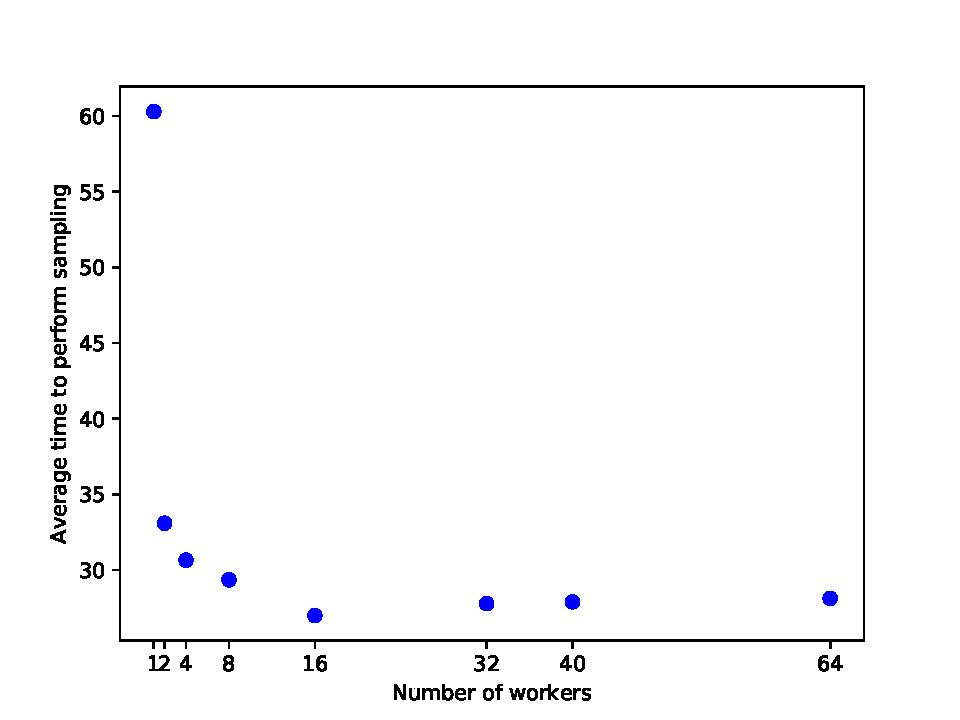
\includegraphics[width=.75\textwidth]{optimizations/workers_experiment.pdf}
    \caption{Average execution time of $500$ steps of the burn-in
        sampling, with varying number of workers. The average values are
        taken over 50 repetitions of the experiment. The model being
        sampled on this experiment contains 5 chemical reactions and 5
        chemical species.}
    \label{fig:parallel_map_sampling}
    \end{center}
\end{figure}



\chapter{Experiments and results}
\label{chap:experiments}
%begin-include

%In this chapter we present experiments of model selection of cell
% signaling pathways. We divide this chapter in two sections; the first
% section presents experiments to compare two model selection software: 
% ABC-SMC and SigNetMS, both of them presented on
% chapter~\ref{chap:model_selection_methods}. We end the first section
% presenting which software had best fit for our experiments. The
% following section presents experiments of model selection as a feature
% selection problem. We will analyze algorithm trace and what is the
% surface induced by the cost function over the search space.

\section{Choosing a Software for Model Selection}
% To choose a software for model selection we did the same experiment as
% girolami
%
% A simple instance of the model selection problem
% -> the correct model is...
% -> then we create other three models
%   - a simplification
%   - an overly complex model
%   - and an incorrect model
% -> the expected result for this experiment is that the correct model
%  has a higher (possibly be the first), and that the incorrect model
%  should be considered the worst. It is also important to see how the
%  software compares models with similar dynamics and with different
%  levels of complexity.
%  
% Results produced by SigNetMS and ABC-SysBio
% -> we proceeded to run both softwares 
% -> compare the ranking of both software
% -> show how the curve fits on both software
% -> show that there is some parameter value convergence on SigNetMS

To choose between SigNetMS and ABC-SysBio, we performed a model
selection experiment. This experiment, originally performed on the work
of Vyshemirsky and Girolami~\cite{Vyshemirsky2007}, consists in creating
artificial experimental data from a model of cell signaling pathway, and 
then selecting between four different models, including the correct one.
Using SigNetMS and ABC-SysBio we should be able to create a ranking of
the four models, in which we expect to see as the best, the model we
used to create the experimental data. More than that, we should analyze
the produced results to check if simpler models are preferred over
complex models; we should also check if the simulations produced by the
models, with the estimated sample of the posterior distribution of
parameters, approximates experimental data.

\subsection{A simple instance of the model selection problem}
\begin{figure}[h]
\begin{center}
    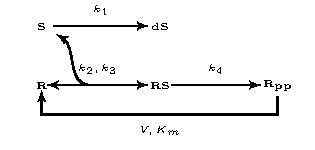
\includegraphics[width=.75\textwidth]{experiments/diagrams/bioinformatics_model1.pdf}
    \caption{A diagram that represents the correct model our simple
model selection experiment. This model represents a common motif, and
has S and Rpp as input and output, respectively. This model contains
five reactions: the decay of S to dS with $k_1$ as reaction rate
constant; the reversible reaction $\ce{S + R <=>[$k_1$][$k_2$] RS}$; the
first order reaction $\ce{RS ->[$k_4$] Rpp}$; and the Michaelis-Menten
reaction $\ce{A ->[$V, K_m$] B}$.}
    \label{fig:experiments:girolami_model1}
    \end{center}
\end{figure}

We start our model selection problem with the correct model, which is 
a signalling pathway composed by five reactions and five chemical 
species. Figure~\ref{fig:experiments:girolami_model1} shows a diagram
with this model. This model represents a common motif, and it has as the 
input signal the chemical species S, and as the output the chemical 
species Rpp; the experimental measurement used is the concentration of 
the output chemical species, which we donote as [Rpp].


In this experiment, for the sake of simplicity, we neglect the units of 
reaction rates constants and initial concentrations. The initial 
concentrations used are:  S $= 1$, R $= 1$, dS $= 0$, RS $= 0$, 
R$_{pp} = 0$. To create the experimental data, the reaction rate 
constants we used have the values: 
$k_1 = 0.07$, $k_2 = 0.6$, $k_3 = 0.05$, $k_4 = 0.3$, $V = 0.017$, and
$K_m = 0.3$. It is important to remember that we discard reaction rate
constant values during model selection; initial concentrations, however,
are still provided during this phase. To generate experimental data, we
simulate the dynamics of this model, using these parameter values, on
the time steps of: 2s, 10s, 20s, 40s, 60s and 100s. Three simulations
are created, and to each one of them we add, for each time measurement,
a Gaussian error with mean $0$ and standard deviation $0.01$. A
representation of the three experiment repetitions are showed on 
figure~\ref{fig:experiments:girolami_simulations}.

% TODO: determine the prior distribution used

% insert simulated data here
\begin{figure}
\begin{center}
    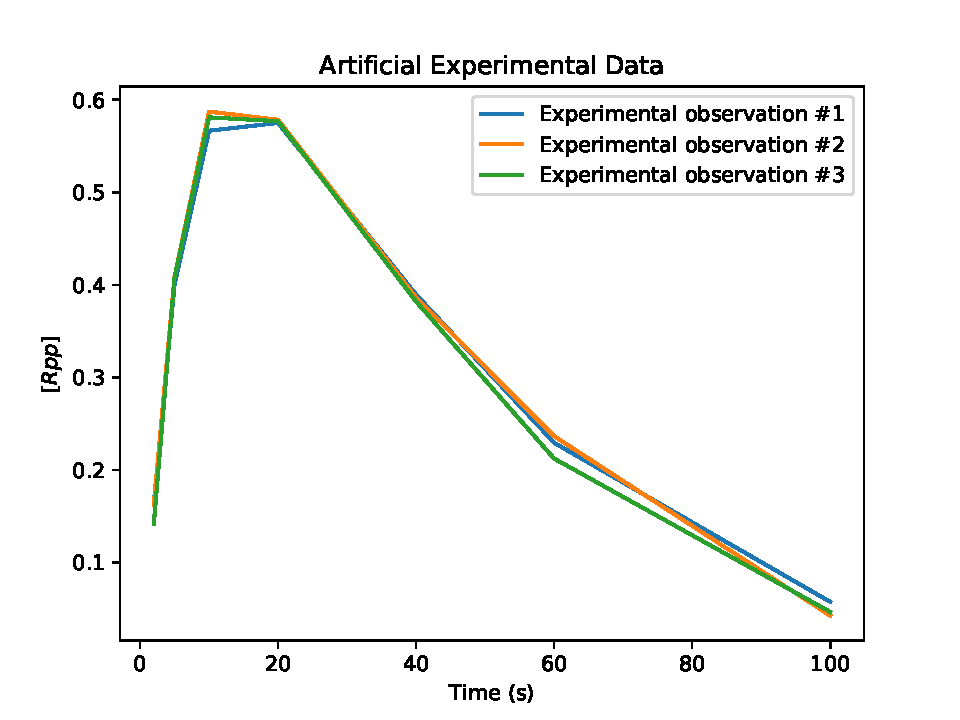
\includegraphics[width=.75\textwidth]{experiments/simulations/girolami_experimental_data.pdf}
    \caption{The dynamics produced by the correct model, with
pre-defined reaction rate constants plus a small Gaussian error, for
each time point. The measurement taken from the model is the
concentration of the Rpp species, which we denote as [Rpp]. We
linearly interpolate the experimental measure points to produce a
continuous dynamics from 2s to 100s.}
    \label{fig:experiments:girolami_simulations}
    \end{center}
\end{figure}

To assess the ranking produced by each of the model selection software,
we compare the first model with three other models (based on the correct
model): a simplified model; an overly simplified model, which should not 
be able to generate the observed dynamics; and, finally, a 
generalization (more complex) model.
Figure~\ref{fig:experiments:girolami_other_models} shows diagrams that
represent the three alternative models.

\begin{figure}[h]
    \centering
    \begin{tabular}{c c}
    \subfigure[simplified model]{
    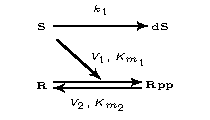
\includegraphics[clip=true,width=.45\linewidth]{experiments/diagrams/bioinformatics_model2.pdf}
    \label{fig:girolami_model2}}
    &
    \subfigure[overly simplified model]{
    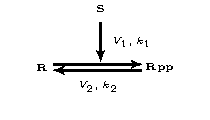
\includegraphics[clip=true,width=.45\linewidth]{experiments/diagrams/bioinformatics_model3.pdf}
    \label{fig:girolami_model3}} 
    \\
\multicolumn{2}{c}{    
    \subfigure[generalization model]{
    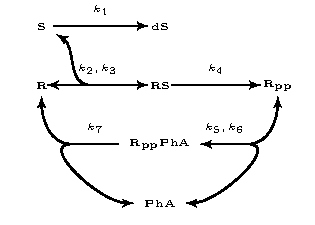
\includegraphics[clip=true,width=.45\linewidth]{experiments/diagrams/bioinformatics_model4.pdf}
    \label{fig:girolami_model4}}
} 
    \end{tabular}
    \caption{The diagrams of three other candidate models, based on the 
correct model that was presented before on 
Figure~\ref{fig:experiments:girolami_model1}. The 
model~\ref{fig:girolami_model2} is a simplification where we neglect the
chemical species RS, and we use the Michaelis-Menten to represent the
reaction $\ce{R -> Rpp}$ with S working as a catalyst.
Model~\ref{fig:girolami_model3} is the over simplified model, as it
neglects the decay of S; we do not expect this model to reproduce
experimental data, since the constant concentration level of S tend to
continuously produce Rpp, a species that, after 20 seconds, has a
monotonic decreasing concentration. Finally,
Model~\ref{fig:girolami_model4} is a generalization of the correct
model, as it generalizes the reaction $\ce{Rpp -> R}$, as instead of 
using the Michaelis-Menten kinetics, we use the enzymatic reaction 
$\ce{Rpp + PhA <=> RppPhA -> R + PhA}$; even though we expect this model
to be able to reproduce observed dynamics, we also expect that the
complexity of this model gets penalized.
}
    \label{fig:experiments:girolami_other_models}
\end{figure}

% -> the expected result for this experiment is that the correct model
%  has a higher (possibly be the first), and that the incorrect model
%  should be considered the worst. It is also important to see how the
%  software compares models with similar dynamics and with different
%  levels of complexity.

Before talking about results produced by different software, we should
note that this choice of candidate models are made so we can analyze
more than the ability of the software to correctly rank the correct
model as the best model. First, consider that we introduced a spurious
model, represented on figure~\ref{fig:girolami_model3} which neglects a
crucial reaction, making it impossible to reproduce the experimental
data; we expect this model to be ranked last between all models. Then,
there are two options to the correct model, one a simplification, and
the other a generalization. For these models, we expect that the
experimental dynamics are possible, however, we should be observant of
how they are ranked according to their complexity. That is important
because, one of the goals on using a Bayesian approach for model 
selection is that these approaches tend to automatically penalize overly
complex models.

% Comparing results of ABC-SMC and SigNetMS
\subsection{Solving a simple model selection instance using ABC-SysBio
and SigNetMS}
% What is the experiment
% What data the experiment produces;
% What are algorithm parameters we used;
% 1 - marginal likelihood of each model
% 2 - a sample of the posterior

% the input and output
After defining the candidate models and producing the artificial
experimental data, we proceeded to perform the experiment of model
selection. The instance related information provided to SigNetMS and 
ABC-SysBio is the same: a model, with predefined initial concentrations
of chemical species; a set of experiments, with the same time steps, 
with measurements of the concentration of Rpp; and a file containing
prior distributions for each one of the model parameters. It is
important to remember that the output produced by each software is
different. SigNetMS produces an estimative of $p({\bm D} | M)$ and also
a sample of the posterior distribution of parameters $p({\bm \theta} |
M, {\bm D})$ which is, in fact, composed by samples of all power
posterior distributions $p_{\beta}({\bm \theta})$ with values as we
described
on~\ref{sec:creating_an_estimative_of_the_marginal_likelihood}.
ABC-SysBio, on the other hand, produces an estimatives of $p({\bm
\theta}, M | {\bm D})$ that might be closer to this target distribution
on each iteration. Note that in this experiment, we need to run SigNetMS
for every model, while on ABC-SysBio we only need to run the software
once for all four candidate models.

The prior distribution of parameters are the same as used by Vyshemirsky
and Girolami~\cite{Vyshemirsky2007}. All model parameters priors are
Gamma(1, 3), where the first and second arguments are shape and scale. 
Gamma and Lognormal distributions are often used as prior for parameters 
because they have a zero probability density for negative values.
% what are algorithm parameter values used

For ABC-SysBio we decided to use its feature of automatically choosing
the schedule of threshold values, which is based on the acceptance of
produced individuals on each iteration. For SigNetMS, we used the
following parameters values: 15000 iterations of the naive burn-in, and
5000 iterations of the posterior shaped burn-in, with 1000 iterations
between covariation matrix rescales, and 3000 iterations of the
Populational MCMC. We used an empiric approach to determine these
parameter values, observing similar results when the number of
iterations are greater than these.

\subsubsection{The ranking produced by ABC-SysBio and SigNetMS}
The ABC-SysBio run created 26 populations of parameter values, each of 
them with 100 individual parameters values. At the last iteration, the 
algorithm stopped with $\epsilon = 1$ and the following estimates: 
\begin{itemize}
    \item{$\hat{p} (M = \text{Correct Model} | {\bm D}, \epsilon = 1) =
        0.005$;}
    \item{$\hat{p} (M = \text{Simplified Model} | {\bm D}, \epsilon = 1)
        = 0.014$;} 
    \item{$\hat{p} (M = \text{Incorrect Model} | {\bm D}, \epsilon = 1)
        = 0.976$;}
    \item{$\hat{p} (M = \text{Generalization Model} | {\bm D}, \epsilon
        = 1) = 0.003$.}
\end{itemize}
These estimates induces the ranking 3, 2, 1, 4.

After running the SigNetMS software four times, one for each model, we
were able to get the following estimates:
\begin{itemize}
    \item{$\log \hat{p}({\bm D} | M = \text{Correct Model}) = 26$}
    \item{$\log \hat{p}({\bm D} | M = \text{Simplified Model}) = 21$}
    \item{$\log \hat{p}({\bm D} | M = \text{Incorrect Model}) = -1$}
    \item{$\log \hat{p}({\bm D} | M = \text{Generalization Model}) =
        19$}
\end{itemize}

% subsubsection Comparing the produced ranking
\subsubsection{Comparing the ranking produced by ABC-SysBio and SigNetMS}
Before comparing the model ranking produced by ABC-SysBio and SigNetMS,
we should state that the ranking achieved by Vyshemirsky and 
Girolami~\cite{Vyshemirsky2007}, on the original work that introduced
this instance, is: Correct Model $\prec$ Generalization Model $\prec$
Simplified Model $\prec$ Incorrect Model. On this work, a methodology
similar to SigNetMS was used.

On ABC-SysBio results, we see that the Correct Model was not ranked
first, and, surprisingly, the Incorrect Model was ranked first. More
than that, when the algorithm stopped, other candidate models were
considered with low probability of being the ``true'' model, and
therefore we cannot strongly state a ranking between the other three
candidates.

On SigNetMS results, we see that the Correct Model was ranked first and 
the Incorrect Model is ranked last as expected. For these two models,
SigNetMS results are equal to the results of Girolami and Vyshemirsky,
and for the other two models, the ranking is the opposite. On SigNetMS,
we ranked the Simplified Model as better than the Generalization Model.
It is important to note here that, in fact, the Generalization Model,
which is more complex, was actually ranked worse than the Correct Model;
that is an evidence that this approach does penalize the complexity of
models.

% subsubsection Analyzing the distribution of posteriors
\subsubsection{Analyzing the posterior distributions produced by
ABC-SysBio and SignetMS}
If we consider only the ranking produced, there are indications that 
SigNetMS is a better choice for our application. However, we should also
take into account other output information produced by both software, 
relative to the distribution of model parameters. ABC-SysBio algorithm 
produces in every iteration a population of parameters that, when 
applied to an specific model, creates a simulation that is at most 
epsilon distant to the experimental measurements, with decreasing 
epsilon as the iteration number grows. SigNetMS, on the other hand, 
produces samples of forty power posterior distributions 
$p_\beta({\bm \theta})$, and although there is no threshold like there 
is on ABC-SysBio, we expect that the closer the value of $\beta$ is to 
$1$, the closer should be the produced simulation to the experimental 
measurements; this is explained by the fact that the power posterior 
distributions $p_0({\bm \theta})$ and $p_1({\bm \theta})$ are, 
respectively, the prior and posterior distribution of parameters.

% One way we could analyze data is looking at the produced simulations
A possible approach to analyze the produced parameters is to simulate
models with those parameter and create simulations to be compared with
the experimental measurements. For ABC-SysBio, in a population of 100
parameters, including the model indicator as one of the parameters, we
are able to simulate and visualize the generated experimental 
measurements for all individuals; on SigNetMS, on the other hand, the 
number of parameter values produced is much greater, than a randomly 
chosen subset of parameters should be enough. With such experiment, we 
are then able to identify what dynamics were created on the candidate 
models according to the estimated posterior distribution of parameters. 

On  figure~\ref{fig:girolami_allmodel_abc} we present the dynamics of 
sampled parameters of the last iterations of the ABC-SysBio run. We can
see on this figure that ABC-SysBio could not produce a set of parameter
values that allows the model to represent the dynamics observed on the
experiment. More than that, we can see that the incorrect model had the
best fit, and the dynamics produced by the sampled parameters induces a
nearly stationary dynamics of $[Rpp]$, with intermediary values of
concentration. With these results, we can understand that the ranking
produced by ABC-SysBio is incorrect because the software could not find
suitable parameter values that allow models to approximate the dynamics
observed on experiments.

\begin{figure}[ht]
    \centering
    \begin{tabular}{c c}
    \subfigure[correct model]{
    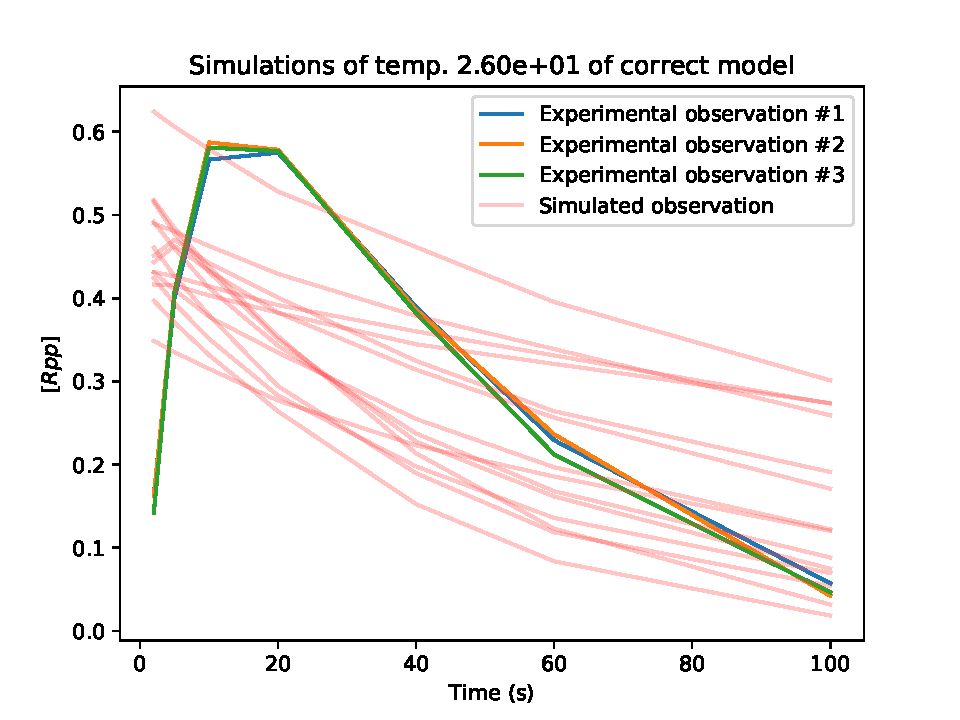
\includegraphics[clip=true,width=.45\linewidth]{experiments/abc_vs_snm/all_model/abc/msimulations_model1_25.pdf}
    \label{fig:girolami_model1_abc}}
    &
    \subfigure[simplified model]{
    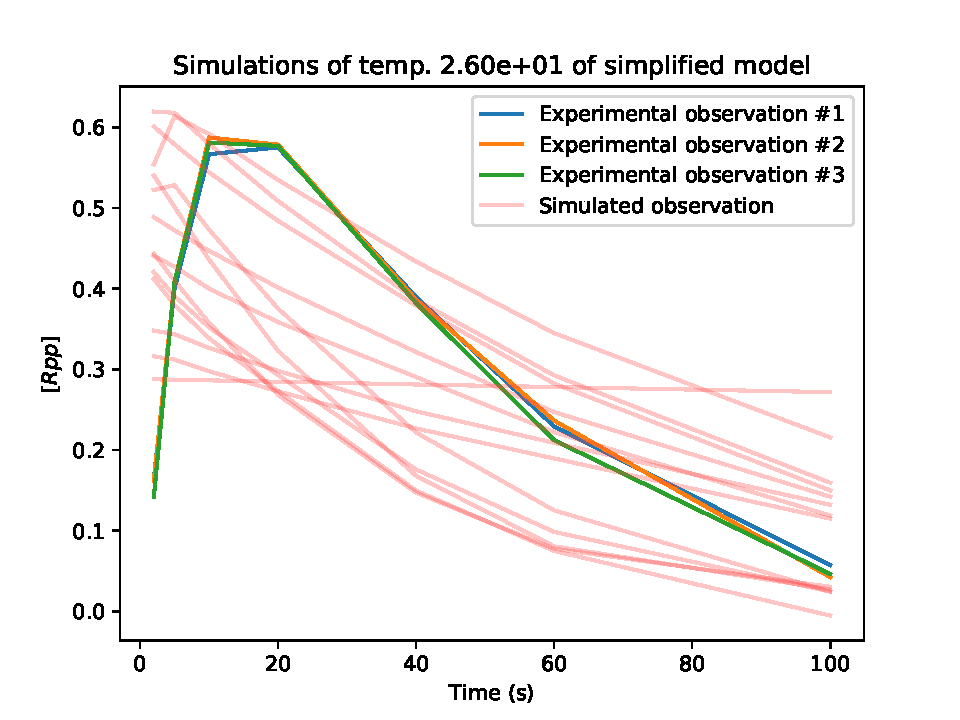
\includegraphics[clip=true,width=.45\linewidth]{experiments/abc_vs_snm/all_model/abc/msimulations_model2_25.pdf}
    \label{fig:girolami_model2_abc}} 
    \\
    \subfigure[incorrect model]{
    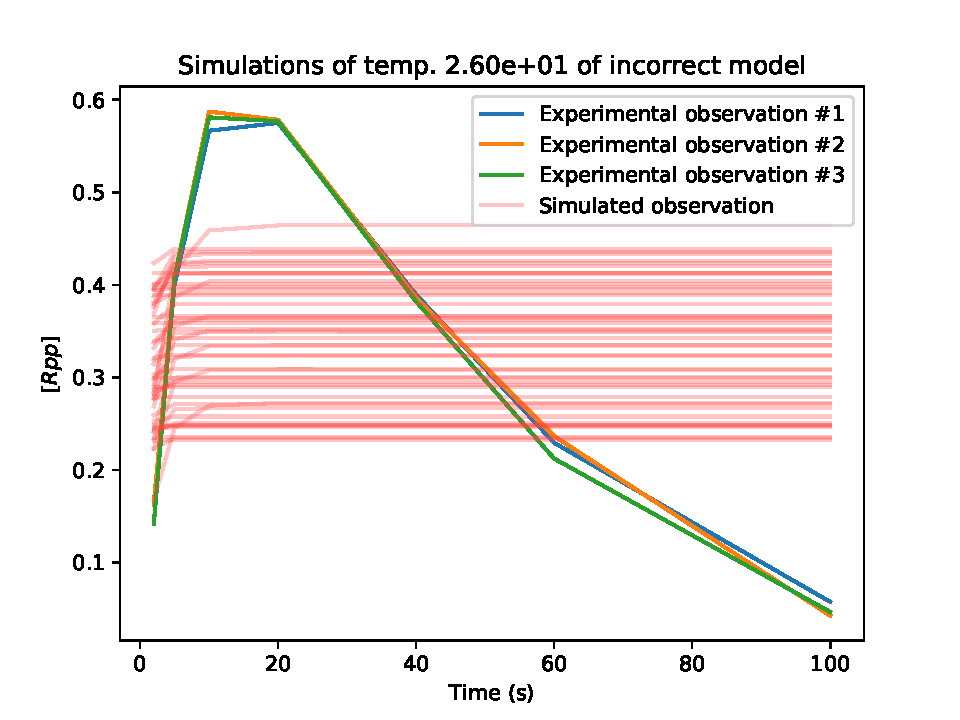
\includegraphics[clip=true,width=.45\linewidth]{experiments/abc_vs_snm/all_model/abc/msimulations_model3_25.pdf}
    \label{fig:girolami_model3_abc}}
&
    \subfigure[generalization model]{
    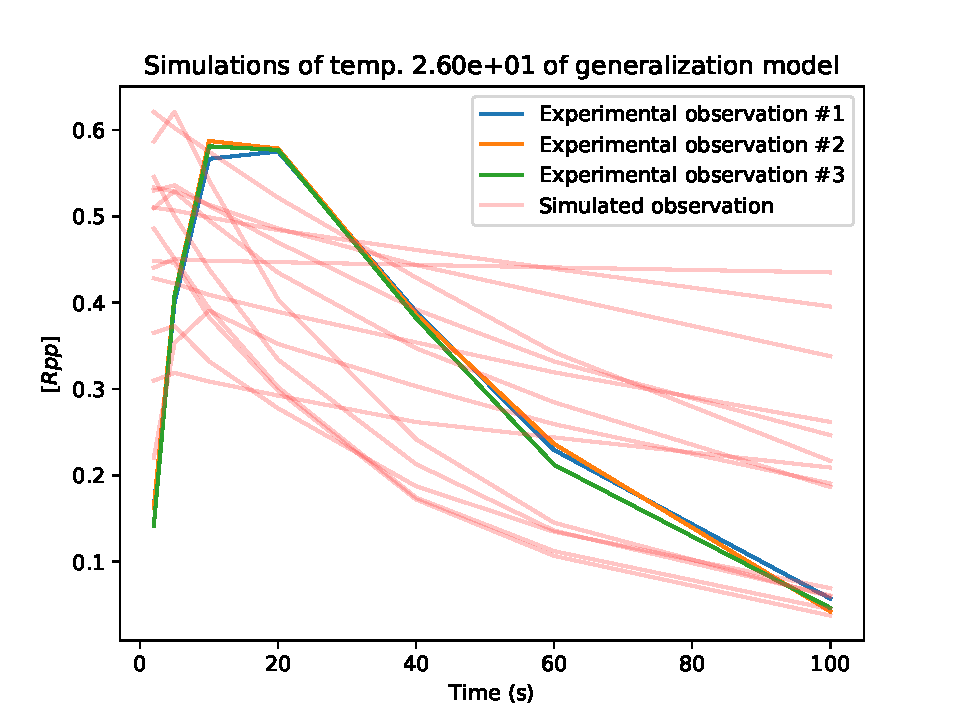
\includegraphics[clip=true,width=.45\linewidth]{experiments/abc_vs_snm/all_model/abc/msimulations_model4_25.pdf}
    \label{fig:girolami_model4_abc}}
    \end{tabular}
    \caption{The simulated dynamics of the four candidate models, using
    parameters generated on the ABC-SysBio software. There are 100
    individuals generated on each iteration of the algorithm, and each
    individual consists of a list of parameter values and a model
    indicator. Because of this, the number of produced simulations is 
    not equal between models, in fact, the better the fit of a model,
    the higher the number of individuals representing such model, and
    therefore, the higher the number of simulations shown. Each red line
    represent an individual simulation, and stronger red lines represent
    overlapping simulations. Lines with blue, yellow and green color
    represent experimental observations.}
    \label{fig:girolami_allmodel_abc}
\end{figure}

On figure~\ref{fig:girolami_allmodel_snm} we present the dynamics of a 
subset of parameters of the posterior distribution (or power posterior 
of $\beta = 1$), for all four candidate models. We can see on this
figure that SigNetMS could not find parameter values that allow the
incorrect model to reproduce experimental observations, which is
expected, and that the three other models candidate models could
closely reproduce the experimental observations. It is also interesting
to observe the dynamics produced by sampled parameters for other values
of $\beta$, which is shown on figure~\ref{fig:girolami_model1_progression_snm},
for the correct model only. Remember that from $\beta = 0$ to 
$\beta = 1$, a sequence of power posterior distributions is constructed 
by SigNetMS, bridging the prior and posterior distributions.

\begin{figure}[ht]
    \centering
    \begin{tabular}{c c}
    \subfigure[correct model]{
    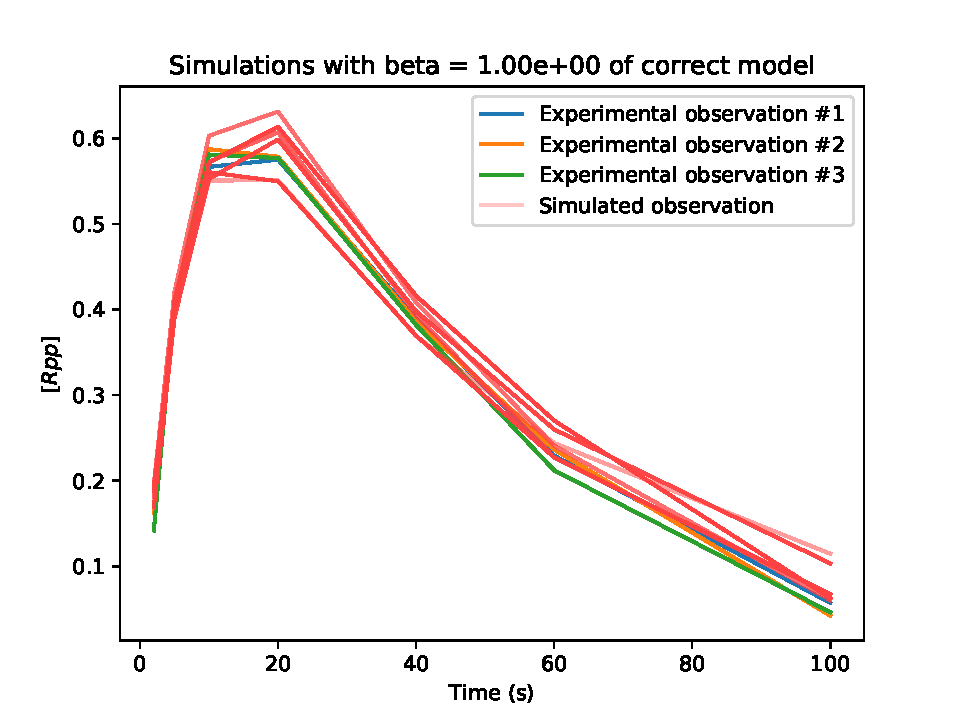
\includegraphics[clip=true,width=.45\linewidth]{experiments/abc_vs_snm/all_model/snm/msimulations_model1_39.pdf}
    \label{fig:girolami_model1_snm}}
    &
    \subfigure[simplified model]{
    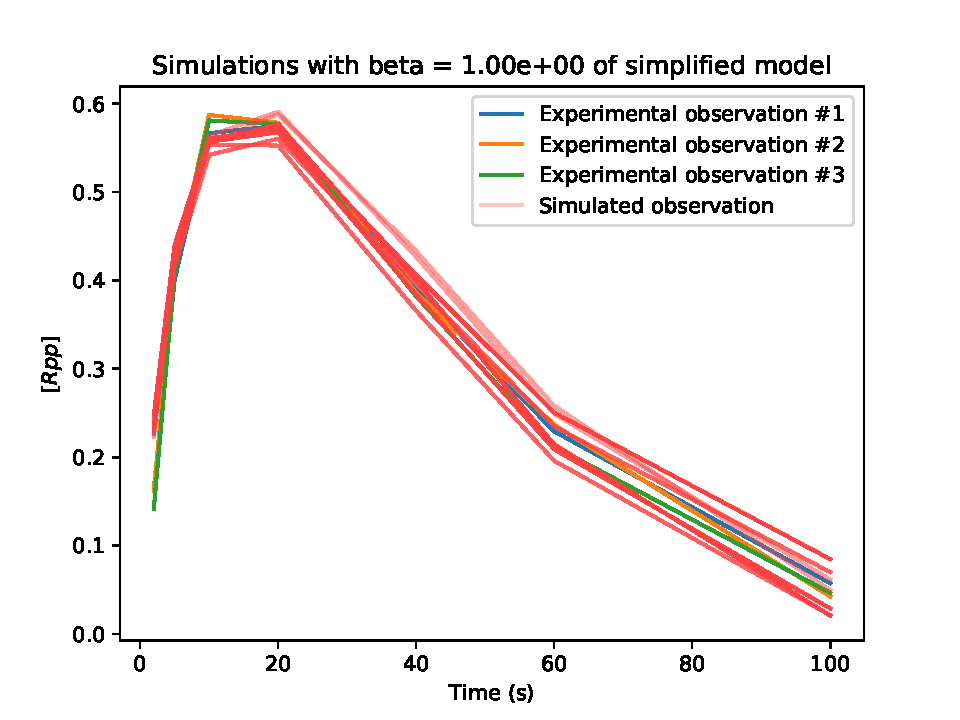
\includegraphics[clip=true,width=.45\linewidth]{experiments/abc_vs_snm/all_model/snm/msimulations_model2_39.pdf}
    \label{fig:girolami_model2_snm}} 
    \\
    \subfigure[incorrect model]{
    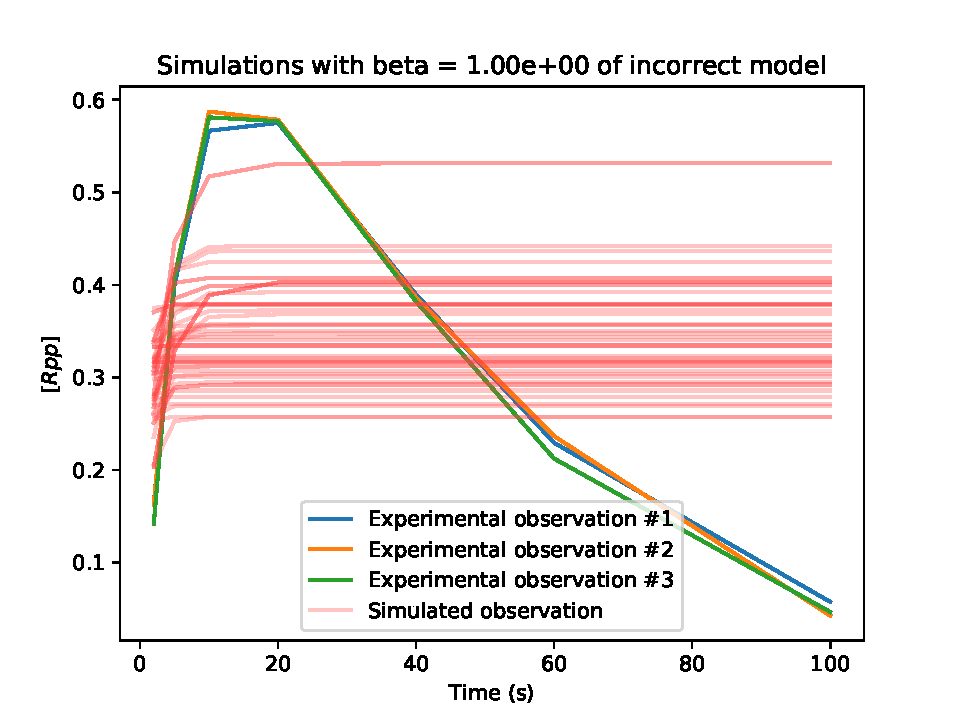
\includegraphics[clip=true,width=.45\linewidth]{experiments/abc_vs_snm/all_model/snm/msimulations_model3_39.pdf}
    \label{fig:girolami_model3_snm}}
&
    \subfigure[generalization model]{
    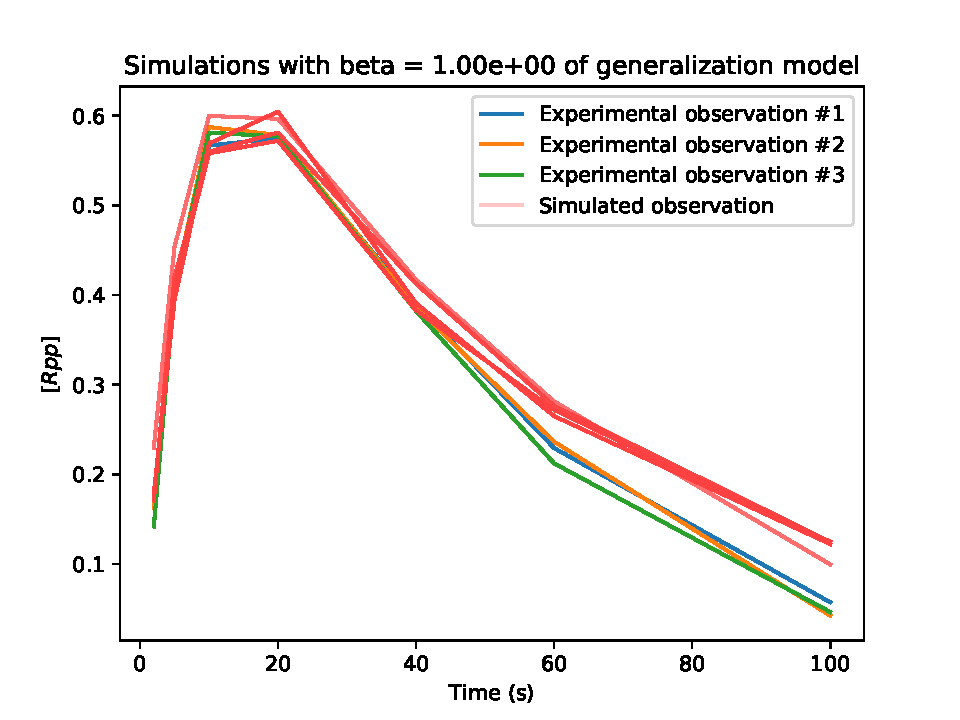
\includegraphics[clip=true,width=.45\linewidth]{experiments/abc_vs_snm/all_model/snm/msimulations_model4_39.pdf}
    \label{fig:girolami_model4_snm}}
    \end{tabular}
    \caption{The simulated dynamics of the four candidate models, using
    randomly chosen subsets of parameters from the sample produced by
    SigNetMS of the power posterior distribution of $\beta = 1$, which
    is the posterior distribution of parameters, $p({\bm \theta} | M,
    {\bm D})$. Red translucent lines represent the simulated dynamics, 
    using the sampled parameters, and stronger lines represent
    overlapping simulations. Lines with blue, yellow, and green color
    represent experimental observations.}
    \label{fig:girolami_allmodel_snm}
\end{figure}

\begin{figure}[ht]
    \centering
    \begin{tabular}{c c}
    \subfigure{
    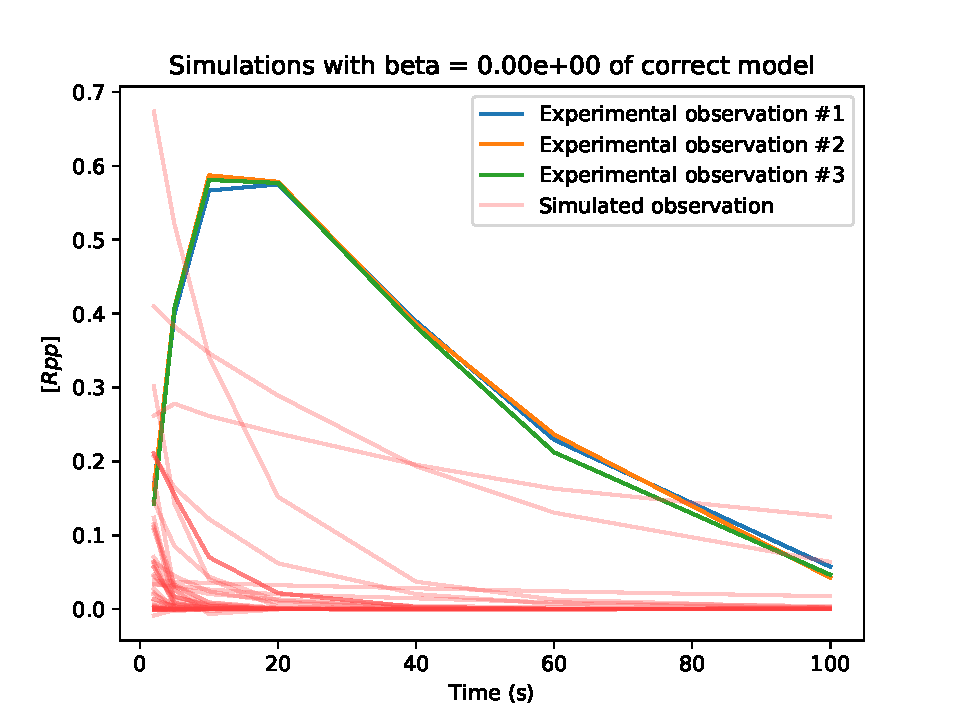
\includegraphics[clip=true,width=.45\linewidth]{experiments/abc_vs_snm/all_model/snm/msimulations_model1_0.pdf}
    \label{fig:girolami_model1_0_snm}}
    &
    \subfigure{
    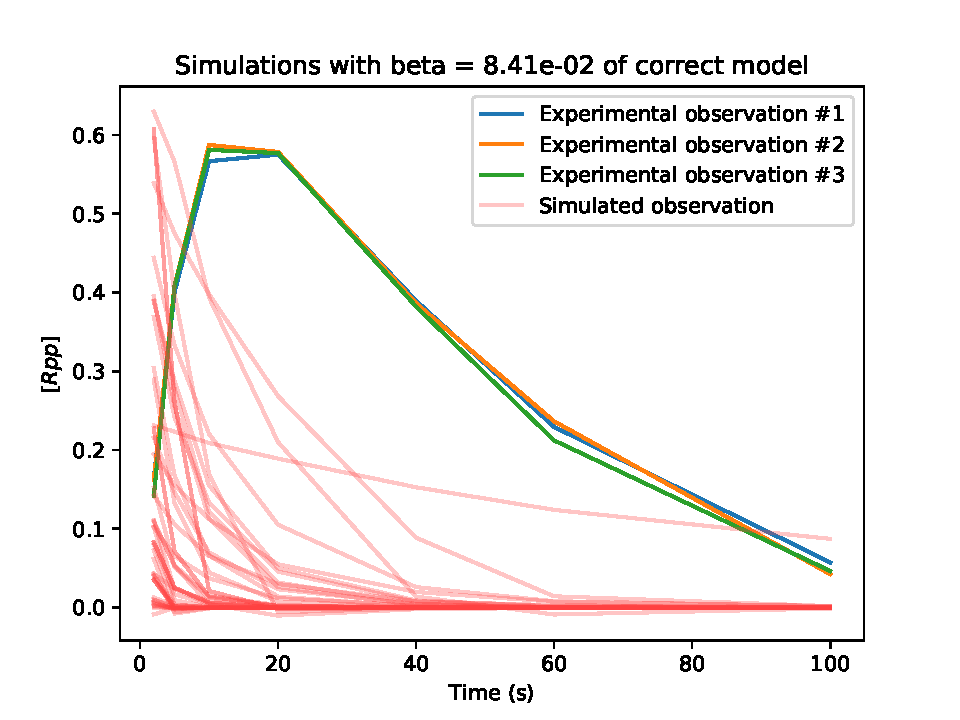
\includegraphics[clip=true,width=.45\linewidth]{experiments/abc_vs_snm/all_model/snm/msimulations_model1_21.pdf}
    \label{fig:girolami_model1_1_snm}} 
    \\
    \subfigure{
    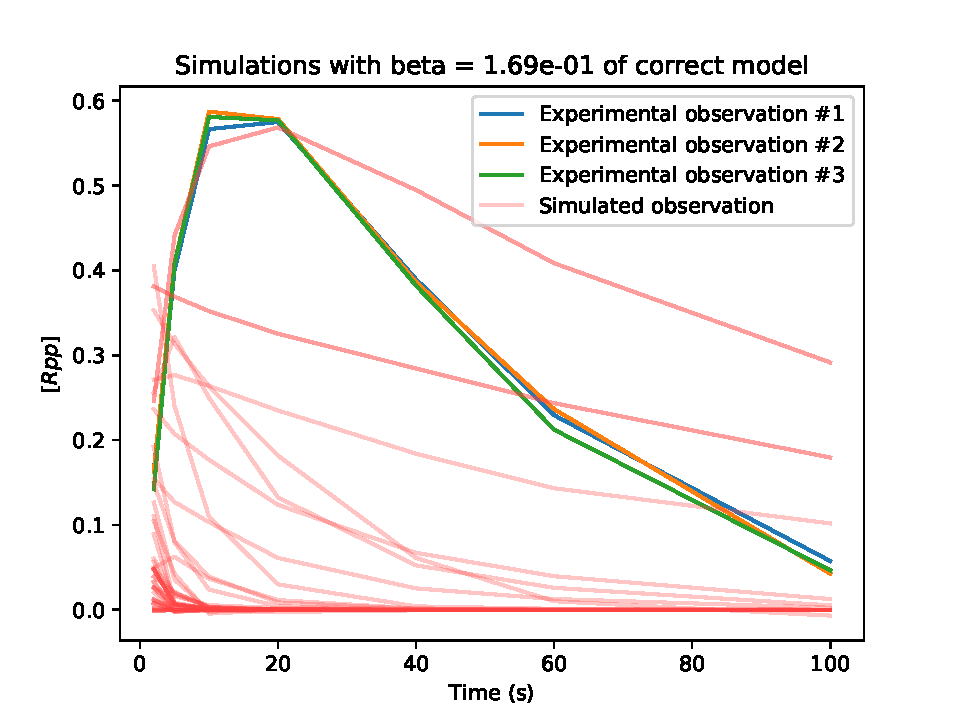
\includegraphics[clip=true,width=.45\linewidth]{experiments/abc_vs_snm/all_model/snm/msimulations_model1_25.pdf}
    \label{fig:girolami_model1_2_snm}}
&
    \subfigure{
    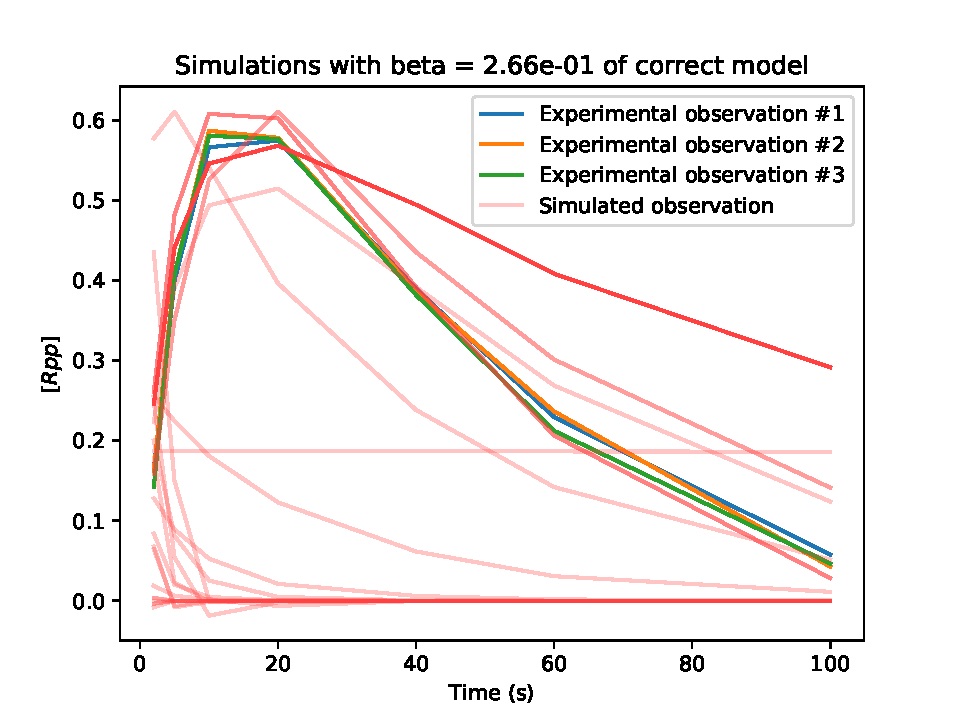
\includegraphics[clip=true,width=.45\linewidth]{experiments/abc_vs_snm/all_model/snm/msimulations_model1_28.pdf}
    \label{fig:girolami_model1_3_snm}}
    \\
    \subfigure{
    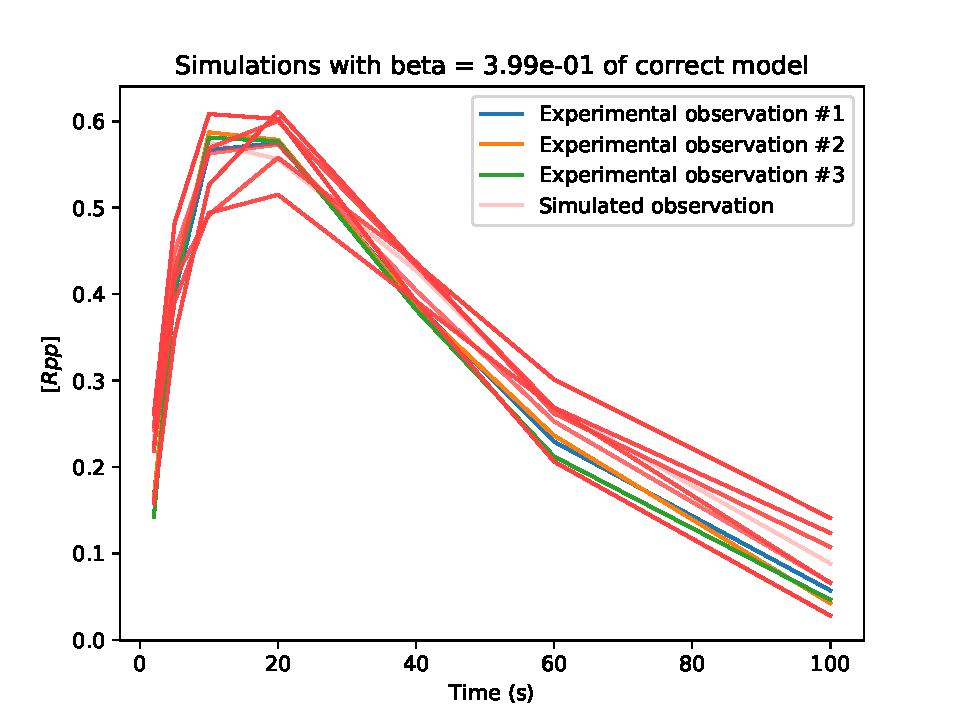
\includegraphics[clip=true,width=.45\linewidth]{experiments/abc_vs_snm/all_model/snm/msimulations_model1_31.pdf}
    \label{fig:girolami_model1_2_snm}}
&
    \subfigure{
    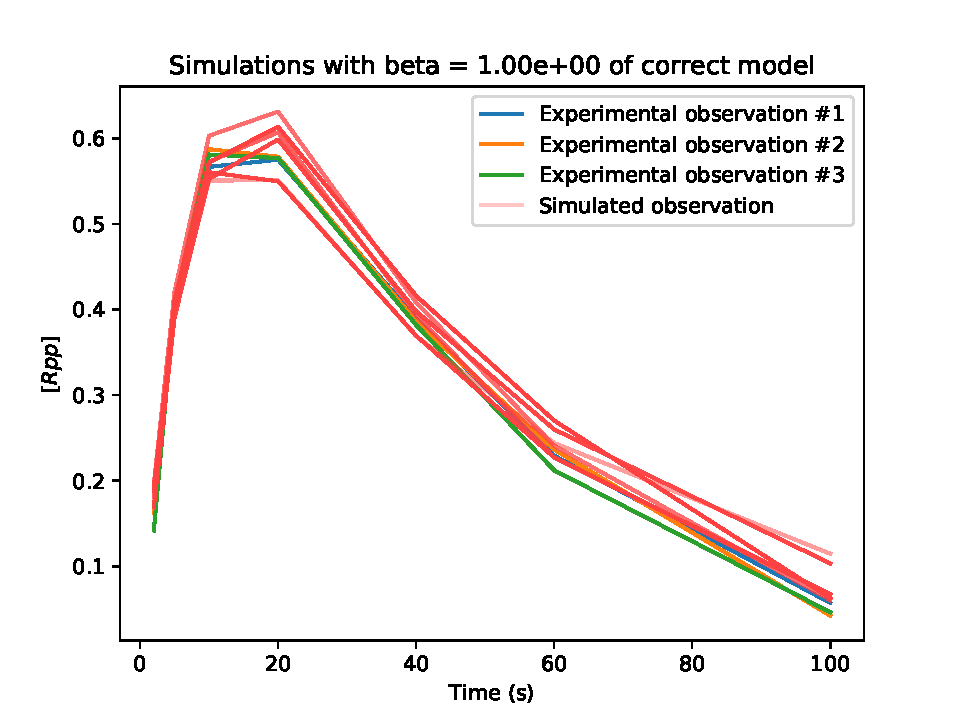
\includegraphics[clip=true,width=.45\linewidth]{experiments/abc_vs_snm/all_model/snm/msimulations_model1_39.pdf}
    \label{fig:girolami_model1_3_snm}}
    \end{tabular}
    \caption{The dynamics induced by samples of different power
    posterior distributions of parameters of the correct model. The
    value of $\beta$ increases from left to right and from top to
    bottom. We can observe how the curve of simulations progressively
    fits the curve of experimental observations.}
    \label{fig:girolami_model1_progression_snm}
\end{figure}

The ranking and the simulations indicate that SigNetMS is more
appropriate for our applications. To further investigate the results
produced by this software, we also created plots of approximations of
the produced power posterior samples, presented on 
figure~\ref{fig:girolami_model1_progression_snm}. These density function
estimates were created using the {\tt distplot} function of the Seaborn
Python package, which uses Gaussian Kernel Densinty Estimate (KDE) to
provide an estimation of the density function given a sample of such
distribution. The presented figure shows estimated power posterior
distributions, with different values of $\beta$, for the $k_1$ parameter
of the correct model, which had value $0.07$ when artificial
experimental data was created. We can see that as we increase the value 
of $\beta$, the posterior distribution concentrates on values around the
``true'' value of the parameter. It is also interesting to see that
although the estimated posterior is not necessarily centered on the 
``true'' value, the created simulations do approximate the experimental
observations.

\begin{figure}[ht]
    \centering
    \begin{tabular}{c c}
    \subfigure{
        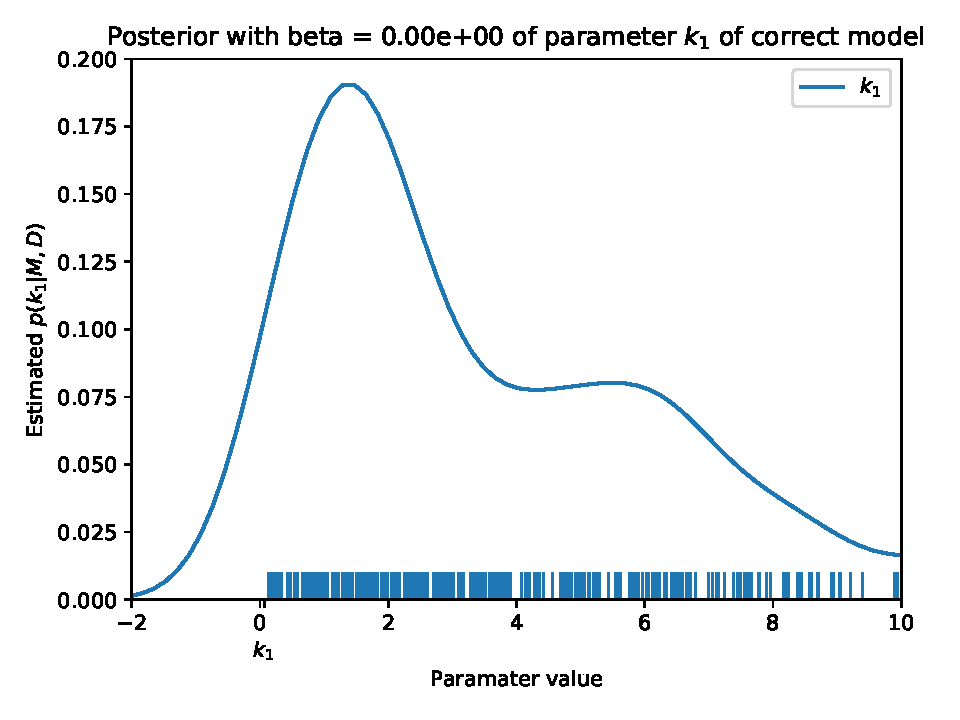
\includegraphics[clip=true,width=.45\linewidth]{experiments/abc_vs_snm/parameters_snm/model1_0_p0_k_1.pdf}
    \label{fig:girolami_model1_0_parameters}}
    &
    \subfigure{
    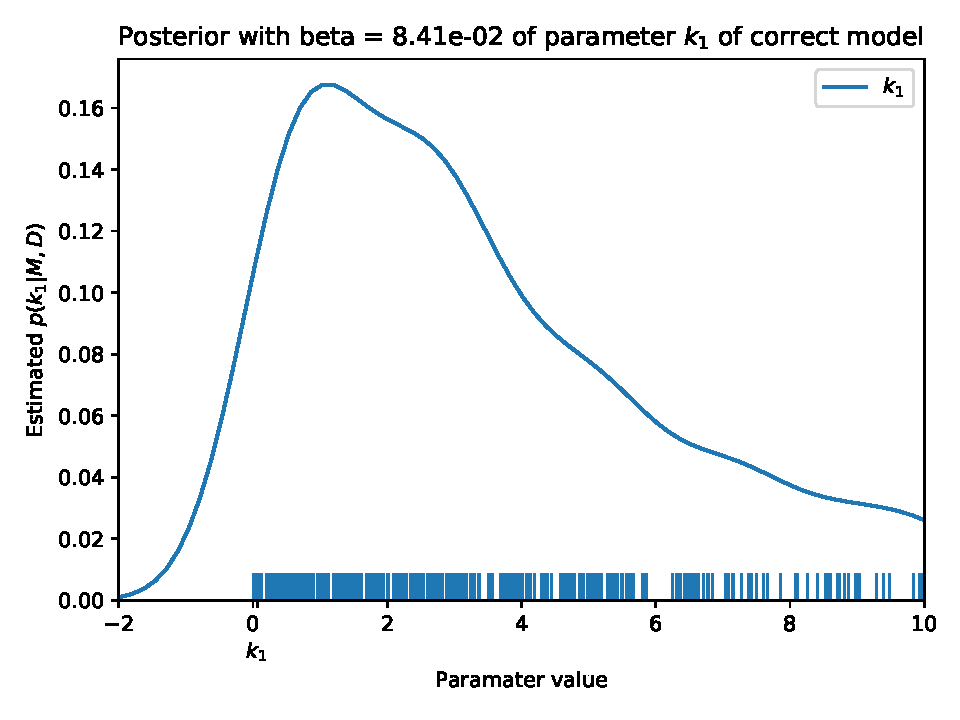
\includegraphics[clip=true,width=.45\linewidth]{experiments/abc_vs_snm/parameters_snm/model1_21_p0_k_1.pdf}
    \label{fig:girolami_model1_1_parameters}} 
    \\
    \subfigure{
    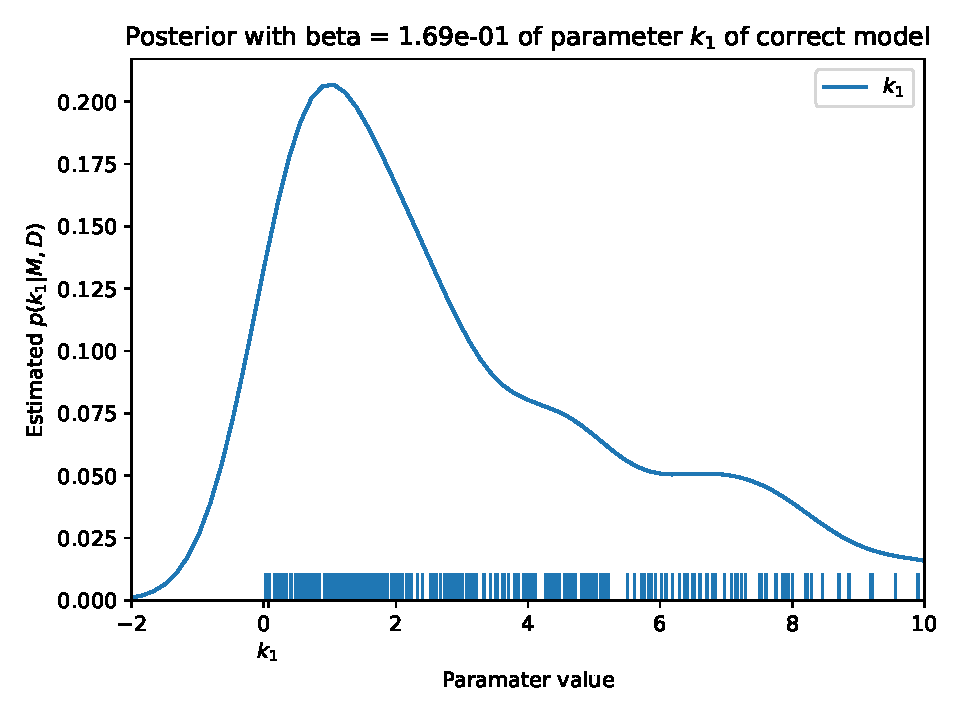
\includegraphics[clip=true,width=.45\linewidth]{experiments/abc_vs_snm/parameters_snm/model1_25_p0_k_1.pdf}
    \label{fig:girolami_model1_2_parameters}}
&
    \subfigure{
    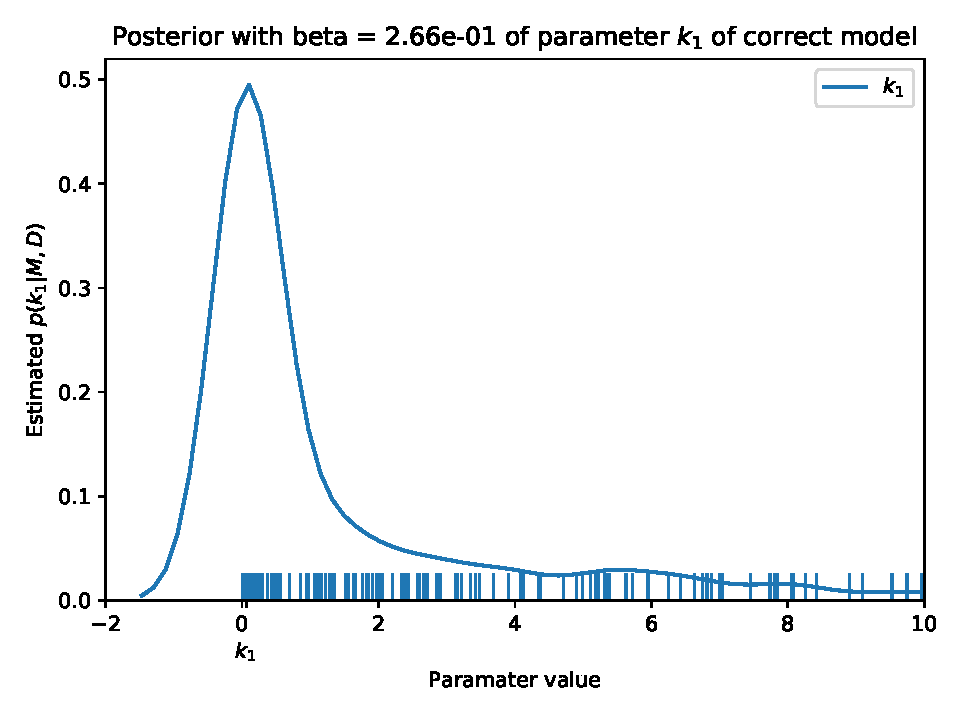
\includegraphics[clip=true,width=.45\linewidth]{experiments/abc_vs_snm/parameters_snm/model1_28_p0_k_1.pdf}
    \label{fig:girolami_model1_3_parameters}}
    \\
    \subfigure{
    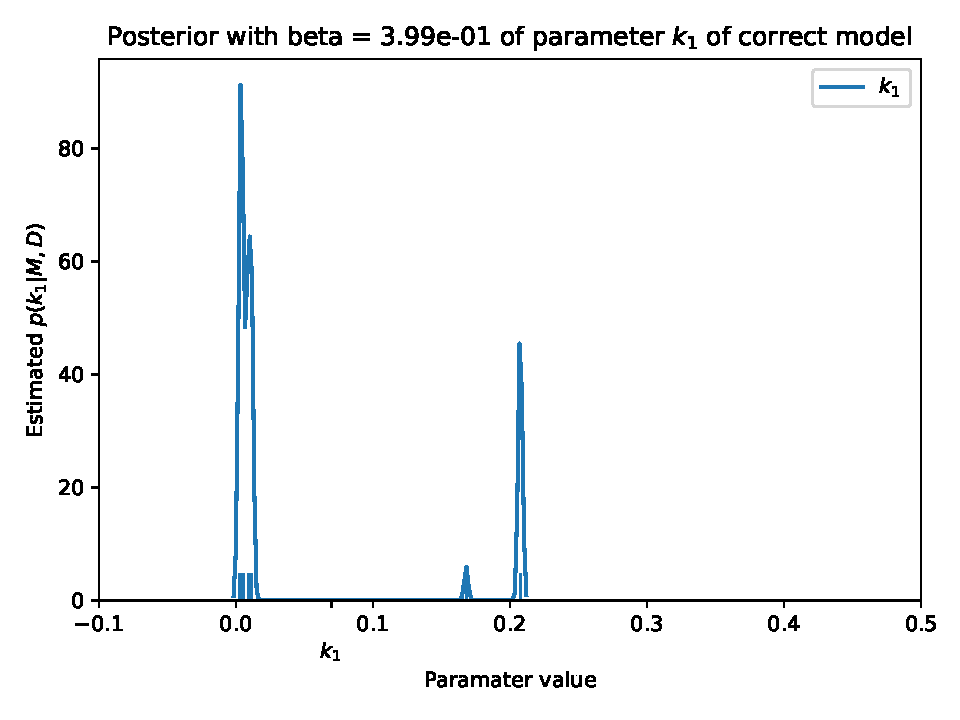
\includegraphics[clip=true,width=.45\linewidth]{experiments/abc_vs_snm/parameters_snm/model1_31_p0_k_1.pdf}
    \label{fig:girolami_model1_2_parameters}}
&
    \subfigure{
    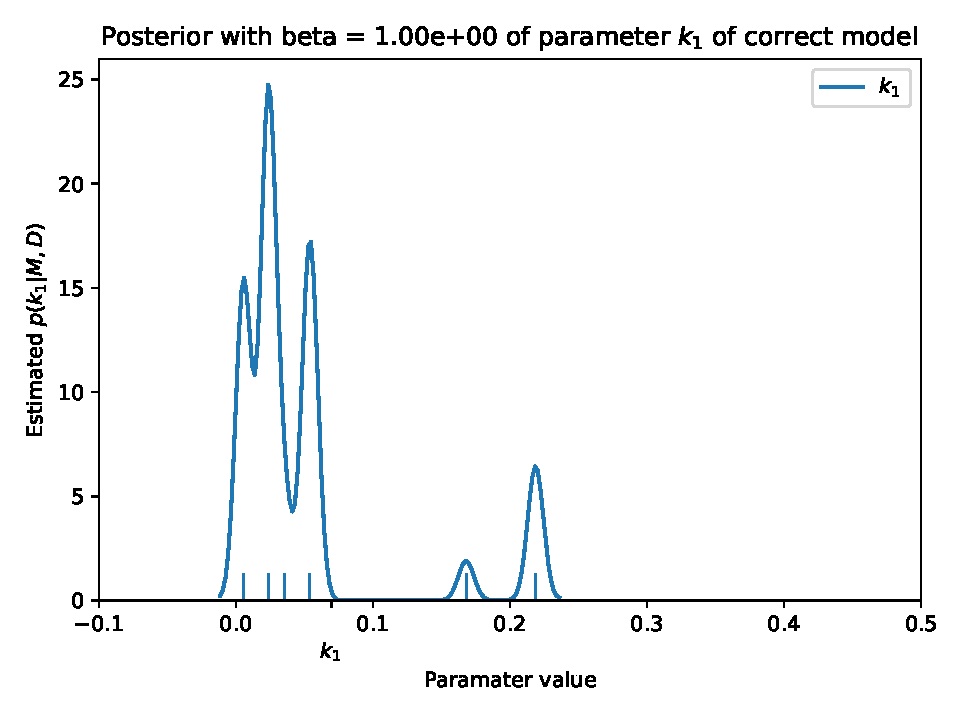
\includegraphics[clip=true,width=.45\linewidth]{experiments/abc_vs_snm/parameters_snm/model1_39_p0_k_1.pdf}
    \label{fig:girolami_model1_parameters}}
    \end{tabular}
    \caption{Approximation of the power posterior distribution of the 
    samples created by SigNetMS of parameter $k_1$ of the correct model.
    We show on this graph the estimated distribution of six different
    power posteriors, with increasing value of $\beta$ from left to
    right, from top to bottom. The approximation of this graph is
    created using {\tt distplot} function of Seaborn package. The value
    used for this parameter on the creation of the experimental data is
    $0.07$, and it is represented on the axis of the plots.}
    \label{fig:girolami_model1_progression_snm}
\end{figure}

\clearpage
\section{Model Selection as a Feature Selection Problem}
% After defining that SigNetMS is our software choice for model
% selection, we will construct another model selection problem instance.
% This time, we intend to use such instance to evaluate the approach
% of solving a model selection problem as a feature selection problem,
% with a Bayesian cost function. Although the instance we use is still 
% small, we will be able to access the surface of possible solutions and 
% get hints of how this surface is induced by the cost function we
% chose.
After defining that SigNetMS is our software choice for model selection,
we are now able to experiment and analyze the approach of solving a 
model selection problem as a feature selection problem, using a Bayesian
approach to define a cost function. To accomplish this, we created
another simple instance of model selection. Although this instance is
still a toy model, we will be able to access the space of possible
solutions and get a glance of the cost surface induced by SigNetMS over
this space.

A feature selection instance can be defined by a pair $(S, c)$ where $S$
is a set of features and $c$ is a cost function that evaluates subsets
of $S$. The space of solution is usually the power set of $S$,
$\mathcal{P}(S)$, and the cost function usually takes values from this 
space to positive real values, $c: \mathcal{P}(S) \to \fieldR$. An
optimal solution is a subset $X \in \mathcal{P}(S)$ such that $c(X) \leq
c(Y), \forall Y \in \powerset (S)$, however, it is important to notice
that the size of the search space grows exponentially with the number of
features and, in practice, with time consuming cost functions, it is
computationally unfeasible use optimal search algorithms. That is
exactly our case, since the cost function we propose to use, based on
SigNetMS, depends on the estimation of multiple power posteriors of
parameters and includes numerous numerical integrations of a system of
ordinary differential equations.

It is often useful to represent the search space with a boolean lattice, 
which is defined by the power set $\mathcal{P}(S)$ and the partial order 
relation $\subseteq$. More than an aid to represent the search space,
the boolean lattice provides a structure that is useful for search
algorithms to define paths and to take advantage of surface of the 
search space, as it is done on algorithms for the U-Curve problem, a 
special case of the feature selection problem where the cost function 
describes a u-shaped curve on every chain of the boolean lattice. The
U-Curve problem is still an NP-hard problem as the feature selection
problem is~\cite{Rei12}, however there are heuristics and optimal
algorithms that can be used on the U-Curve problem to produce a quality
answer (optimal or close to be optimal) with a feasible computational
time. Moreover, one can produce good results using U-Curve algorithms to 
solve a feature selection instance that is not necessarily U-Curve, but
does reproduce u-shaped curves with a few oscillations on chains of the
search space.

In our application, we are going to convert a model selection problem
into a feature selection problem. To do so, we define a set of candidate
reactions $S$ and a base model. Then, we consider that a set of feature
$X \in \powerset (S)$ represents a candidate model composed by the base
model plus the reactions from $X$. The cost function we use is the
marginal likelihood produced by SigNetMS.
Figure~\ref{fig:feature_selection_model_selection} shows an example of
feature selection instance that represents a model selection instance.

\begin{figure}[ht]
\begin{center}
    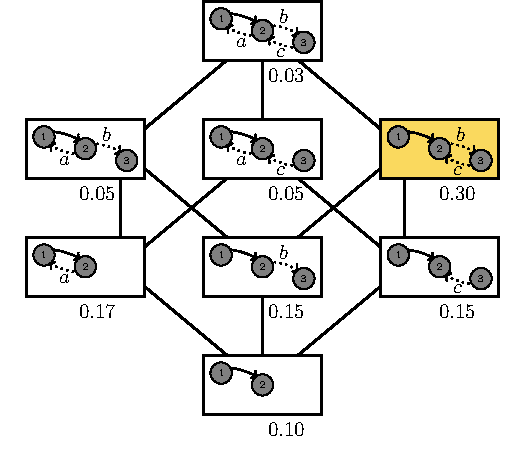
\includegraphics[width=1\textwidth]{experiments/Boolean_lattice_model_selection.pdf}
    \caption{A diagram with the search space and costs of a feature 
    selection problem that represents a model selection problem. Each 
    rectangle represents a subset of the power set of features, were
    reactions from such subset are drawn with dots. Links between 
    rectangles represent the $\subseteq$ relation; that is, two 
    rectangles linked represent two subsets of reactions $X$ and $Y$ 
    such that $X \subseteq Y$ (or $Y \subseteq X$). The set of features 
    is composed by three reactions, $\{a, b, c\}$, inducing the search 
    space with eight elements. The base model is composed by two 
    chemical species, $1$ and $2$ and a reaction between those species, 
    we can see this model at the base of the diagram, on the rectangle 
    that represents the empty set (no reaction are drawn with dots). 
    Each rectangle also represents a candidate model, which is composed 
    by the base model plus the reactions drawn with dots. The number
    below each rectangle represents the score (minus one times the cost)
    of each model. The optimal subset is drawn in yellow and it the
    subset of reactions $\{b, c\}$. Note that this instance is a U-Curve 
    instance, if we consider the cost as minus one times the score: for 
    every chain of rectangles, the cost of the model describes a u 
    shaped curve. As an instance, consider the chain $\emptyset, \{c\} 
    , \{a, c\}, \{a, b, c\}$, which has respectively the costs of
    $-0.10$, $-0.15$, $-0.30$, and $-0.03$.}
    \label{fig:feature_selection_model_selection}
    \end{center}
\end{figure}

After defining the feature selection instance, we will traverse the
search space in two ways. First, we will traverse chains from the empty
set to the complete set, to understand the shape of the cost function as
we increase the number of reactions. Then, we will run the Sequential 
Forward Search algorithm, a heuristic for the feature selection problem,
to try to find a good solution for our model selection problem.


% talk about search algorithms
% talk about the U-Curve problem  

% introduce an example of the boolean lattice

% The feature selection problem is...
% the features are blah,
% the cost function is bleh,

\subsection{Defining the Feature Selection Instance}
% The instance we chose to show is a Ras switch pathway. This pathway...
% This time we also define the correct model, which is shown on Figure.
% We define the space of features as the set of reactions shown on
% Figure.

% We define as a "base model", a simple pathway which has no reactions,
% and for each node of the search space, we consider that such node
% represents the empty model with the reactions present on that node.

% The list of candidate reactions is shown on figure blah
% 

The instance we prepared is based on a Ras switch pathway. Ras
represents a family of proteins that are common on signaling pathways
that participate on cell growth and differentiation. Because of this
participation, Ras proteins that are constantly switched on can play a 
part on some types of cancer. The model we consider for generating 
experiments, which we also call the ``correct'' model is shown on 
Figure~\ref{fig:ras_switch:correct_model}. This model shows a pathway
that decides the state of a Ras protein as switched on, represented by
RasGTP, and as switched off, represented by RasGDP. Five other chemical
species are present on this model, and they have the following initial
concentration: 200 for SOS; 0 for SOS\_allo\_RasGDP and
SOS\_allo\_RasGTP; 900 for RasGDP; 100 for RasGTP; 200 for GEF; and 125
for GAP. Once again, we omit concentration and reaction rate units for
the sake of simplificty. These chemical species interact in eight
different chemical reactions:
\begin{itemize}
    \item{$\ce{SOS + RasGDP ->[k2] SOS\_allo\_RasGDP}$};
    \item{$\ce{SOS\_allo\_RasGDP ->[d2] SOS + RasGDP}$};
    \item{$\ce{SOS + RasGTP ->[k1] SOS\_allo\_RasGTP}$};
    \item{$\ce{SOS\_allo\_RasGTP ->[d1] SOS + RasGTP}$};
    \item{$\ce{RasGTP -> RasGDP}$}, with SOS\_allo\_RasGTP as a
        catalyst, and $k3cat$ and $K3m$ as catalytic constant and
        Michaelis constant, respectively;
    \item{$\ce{RasGTP -> RasGDP}$}, with SOS\_allo\_RasGDP as a 
        catalyst, and $k4cat$ and $K4m$ as catalytic constant and
        Michaelis constant, respectively;
    \item{$\ce{RasGTP -> RasGDP}$}, with GEF as a catalyst, and
        $k6cat$ and $K6m$ as catalytic constant and Michaelis constant,
        respectively;
    \item{$\ce{RasGDP -> RasGTP}$}, with GAP as a catalyst, and
        $k5cat$ and $K5m$ as catalytic constant and Michaelis constant,
        respectively.
\end{itemize}

\begin{figure}[ht]
\begin{center}
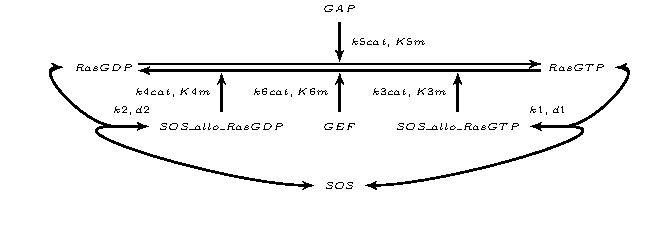
\includegraphics[width=1\textwidth]{experiments/ras_switch/correct.pdf}
\caption{A representation of a Ras switch pathway that we consider as
    the correct model for our model selection experiment. This model
    contains seven chemical species, and eight different chemical
    reactions. Reversible reactions are represented with arrows poiting
    both directions, with reaction rate parameters over the reaction,
    with the forward reaction parameter first and then the parameter of
    the reverse reaction. Michaelis-Menten reactions are represented
    with parameters to the left of the arrow from starting at the
    enzyme, with the catalystic parameter first, and then the Michaelis
    constant.
}
\label{fig:ras_switch:correct_model}
\end{center}
\end{figure}

We used this model to generate an artificial experiment where the
concentration of activated Ras was measured at the time steps of 30,
60, 90, 120, 150, 180, 210, and 240 seconds.
Figure~\ref{fig:ras_switch:experimental_observations} shows a graph of
such experimental measurements. Similarly to the experiment of the 
previous section, those observations were created by simulating the 
correct model and then adding a Gaussian error of mean zero and standard
deviation of 0.01. The reaction rate parameters used to create these
simulations are: k1 $= 1.8e-4$, d1 $= 3$, k2 $= 1.7e-4$, d2 $=0.04$,
k3cat $= 3.8$, K3m $=1.64e3$, k4cat $= 0.003$, K4m $= 9.12e3$, k5cat
$= 0.1$, K5m $= 1.07e2$, k6cat $= 0.01$, and K6m $=1836$ (once again,
remember that we are omitting units for the sake of simplicity).
%<parameter id="k1"    value="1.8e-4"/>
%<parameter id="d1"    value="3.0"/>
%<parameter id="k2"    value="1.7e-4"/>
%<parameter id="d2"    value="0.04"/>
%<parameter id="k3cat" value="3.8"/>
%<parameter id="K3m"   value="1.64e3"/>
%<parameter id="k4cat" value="0.003"/>
%<parameter id="K4m"   value="9.12e3"/>
%<parameter id="k5cat" value="0.1"/>
%<parameter id="K5m"   value="1.07e2"/>
%<parameter id="k6cat" value="0.01"/>
%<parameter id="K6m"   value="1836"/>

\begin{figure}[ht]
\begin{center}
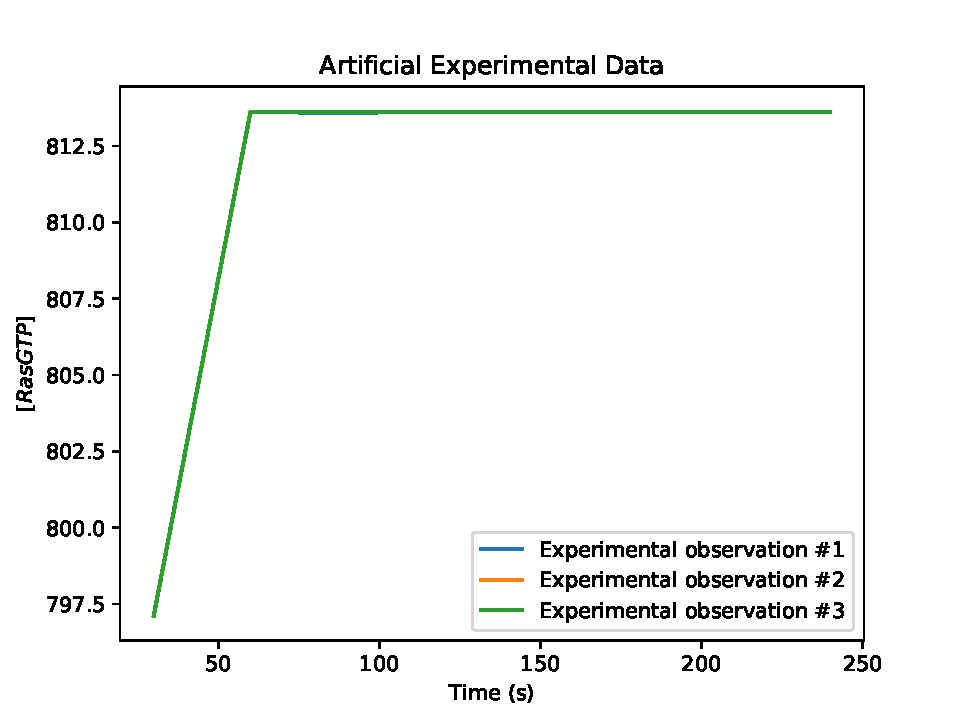
\includegraphics[width=.75\textwidth]{experiments/ras_switch/experiment_plot.pdf}
\caption{Experimental data generated with our correct model for the Ras
    switch pathway. There is a set of three observations being
    represented, however, the time points observations of [RasGTP] are
    close enough that the lines of each experiment overlap. The time
    points considered are 30, 60, 90, 120, 150, 180, 210, and 240
    seconds; the lines are produced with a linear interpolation of
    measurements on these points.}
\label{fig:ras_switch:experimental_observations}
\end{center}
\end{figure}

To construct our search space, we considered as the base of our search
space a trivial model, containing no reactions. For the set of features,
we considered all reactions from the correct model (i.e. the correct
model is present on the search space), plus two other reactions. A
complete list of candidate reactions is shown of
Figure~\ref{fig:ras_switch:features}.


\begin{figure}[ht]
    \centering
    \begin{tabular}{cc}
    \subfigure{
        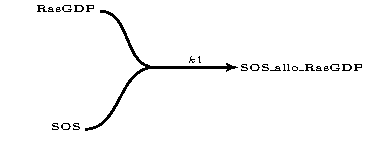
\includegraphics[clip=true,width=.35\linewidth]{experiments/ras_switch/reactions/sos_allo_rasgdp_complexation.pdf}
    }
    &
    \subfigure{
        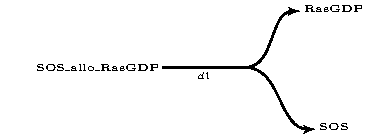
\includegraphics[clip=true,width=.35\linewidth]{experiments/ras_switch/reactions/sos_allo_rasgdp_decomplexation.pdf}
    }
    \\
    \subfigure{
    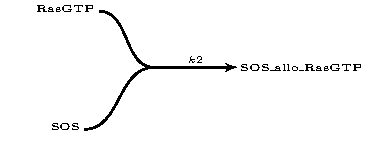
\includegraphics[clip=true,width=.35\linewidth]{experiments/ras_switch/reactions/sos_allo_rasgtp_complexation.pdf}
    }
    &
    \subfigure{
    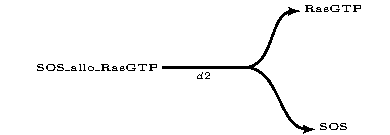
\includegraphics[clip=true,width=.35\linewidth]{experiments/ras_switch/reactions/sos_allo_rasgtp_decomplexation.pdf}
    }
    \\
    \subfigure{
    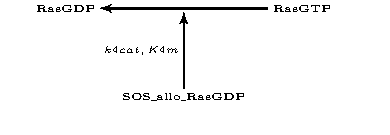
\includegraphics[clip=true,width=.35\linewidth]{experiments/ras_switch/reactions/ras_activation_by_sos_allo_RasGDP.pdf}
    }
    &
    \subfigure{
    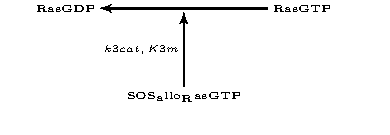
\includegraphics[clip=true,width=.35\linewidth]{experiments/ras_switch/reactions/ras_activation_by_sos_allo_RasGTP.pdf}
    }
    \\
    \subfigure{
    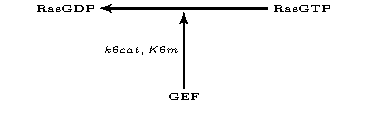
\includegraphics[clip=true,width=.35\linewidth]{experiments/ras_switch/reactions/ras_activation_by_GEF.pdf}
    }
    &
    \subfigure{
    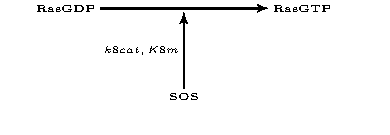
\includegraphics[clip=true,width=.35\linewidth]{experiments/ras_switch/reactions/ras_activation_by_SOS.pdf}
    }
    % TODO: finish this figure
    \end{tabular}
    \caption{Approximation of the power posterior distribution of the 
    $0.07$, and it is represented on the axis of the plots.}
    \label{fig:girolami_model1_progression_snm}
\end{figure}




% Walk through optimal experiment
% SFS experiment
% done!


\chapter{Conclusion}
\label{chap:conclusion}
We will start this chapter with a review of the content presented in 
this dissertation, with some extra discussion of a few specific topics.
After that, we will present the main contributions of this work,
including technological tools and publications. Finally, we will close
this chapter with possibilities of future work related to this
dissertation.


\section{Review of contents of this dissertation}
% Review of the contents of this work
On the Introduction of this text, we presented the main aspects of cell
signaling pathways and how computational models can approximate their
dynamics. After that, we showed how Wu~\cite{Wu15} defined an approach
for model selection of cell signaling pathwyas as a feature selection
problem, and also the main caveats of their approach. With that, we
could state the goal of this project, which is to study and develop a
similar method for model selection using feature selection, where the 
cost function is created with a Bayesian approach, capable of
determining the likelihood of a model producing experimental data.

% Why did we go for that goal?
% hability to input prior knowledge
% auto-penalize complex models

We decided to use a Bayesian approach to construct the cost function
because of its ability to auto penalize overly complex models, avoiding
some sort of ``overfit'' that can occur, characterized by complex models
that have good ability to fit an example of experimental data, but have 
poor generalization performance. Another reason to use a Bayesian
approach is that this approach consider model parameters as random 
variables, which allow the user to input their prior knowledge, and also
to produce a posterior distribution for model parameters. Specially in 
our application, where model parameters are related to the rate 
constants of reactions, using a non deterministic approach to model 
constants is closer to what is seen in the real world; since those 
reactions can occur in a variety of conditions, reaction rate constants
are not fixed constants.

% Ok, then on chapter 2 we revised some content
Before introducing concepts and methodologies we developed in this work,
we reviewed the fundamental concepts necessary to advance in this 
project. On Chapter 2 we conduced this review, presenting concepts
of cell signaling pathways, experimental measurements of those systems, 
and also how to create computational models for them, using system of 
ordinary differential equations. We also introduced the state of the art
methodologies for model selection in the context of cell signaling
pathways and the algorithm of Metropolis-Hastings, to generate samples
of unknown distributions.

% Then we reviewed state of the art model selection
On Chapter 3 we presented a short review of two different methodologies
for evaluating the quality of models. The first methodology, uses an
estimative of the marginal likelihood of a model being the ``correct''
given the experimental data. This estimative is created by sampling from
different power posterior distributions, bridging the prior and
posterior distribution of model parameters; to conduce those
calculations, it is necessary to define a likelihood function. The 
second methodology, uses the concept of Approximate Bayesian 
Computation, and it also produces a sequence samples that for each
iteration approximates better the posterior distribution of parameters.
This last approach however, does not depend on the definition of a
likelihood function. There are available software that apply both
methodology, BioBayes and ABC-SysBio, for the first and second
approaches, respectively.

% Then we produced an almost efficient way to calculate marginal
% likelihoods
After testing both software, BioBayes and ABC-SysBio, we found that
BioBayes would be cumbersome to use as part of a feature selection cost
function. We then decided to produce a new software to estimate marginal
likelihood of models, and we called it SigNetMS. On Chapter~4 we
presented the main procedures we needed to build for this software. We
highlighted the sampling procedure as a computationally expensive
procedure, mainly because of the multiple numerical integrations
necessary to build the sample. We discussed how we decided for a
numerical integration software, since producing one ourselves was not
possible in the scope of this project. We discussed how we could
optimize our process in order to make more efficient calls of the
integrator, using symbolic mathematics to represent our system. Finally,
we presented how we managed to sample from multiple power posterior
distributions, using parallelization.

% We then compared ABC-SysBio to SigNetMS
With the implementation of SigNetMS, we could then compare both
methodologies to evaluate models: based on the marginal likelihood
estimation, using SigNetMS, and based on Approximate Bayesian
Computation, using ABC-SysBio. To compare them, we used a simple model
selection instance, with four models including a ``correct'' model, used
to generate artificial experimental measurements. As the result we
could see that SigNetMS produced a better ranking of models compared to
ABC-SysBio. We could also see that SigNetMS evaluated a simpler model as
better than a model with similar ability to reproduce experimental data,
but with higher complexity; which is an evidence that, in fact, the
Bayesian approach does penalize the complexity of models.

% And finally, we experimented on a small instance
Since SigNetMS produced better results on the simple model selection
instance, we used this software in our next experiment: a model
selection problem solved as a feature selection problem. To build this
instance, we defined a ``correct'' model of a Ras switch to generate
artificial experimental data, and a set of candidate reactions
(including all reactions of the correct model). Then, we created a
feature selection instance where the set of features is the set of
candidate reactions, and the cost of a subset is minus one times the
marginal likelihood of a model with such subset. To conduce the search,
we used the Sequential Forward Selection heuristics, and as a result, we
got a subset with five features, different from the ``correct'' subset,
with eight features. We produced plots that indicate that for both
``correct'' and found subset, the produced sample does make the model
reproduce the experimental data; however, the cost of the ``correct''
model was higher, which indicates that its complexity was penalized,
since a simpler model could reproduce its measured dynamics.

% And what did we learn after all?
Finally, with this last experiment, we could actually confirm that the
Bayesian approach does penalize complex models. More than that, we could
confirm that the sample produced by SigNetMS, when possible, does
approximate the model dynamics to the experimental measurements
dynamics. However this results indicates that SigNetMS could be used for
other examples of model selection, we should also highlight that our
experiment was small, and further experimentation is needed to improve
the SigNetMS software, preparing it for larger and harder instances.

\section{Contributions of this dissertation}
% Contributions of this work
% -> technological
% -> participation in congresses where we presented this work
%   -> Rocky 2019
%   -> São Paulo School of Data Science
% -> advanced school of mathematics
The main contributions during this work are the following:

% TODO: organize with technological or experience contributions

\begin{itemize}
\item{The implementation of SigNetMS, a free software that allows
    evaluating the quality of models, generating an estimative of the
    marginal likelihood of a model, and also a posterior sample of model
    parameters.}
\item{The comparison of two Bayesian approaches for model selection:
    using marginal likelihood and approximate Bayesian computation.
    Conduced on Chapter~\ref{chap:experiments}.}
\item{The experimentation of a feature selection approach for model
    selection, using a Bayesian cost function, conduced on
    Chapter~\ref{chap:experiments}.}
\item{The participation at the São Paulo School of Advanced Science on 
    Learning from Data, as a volunteer, including a five minute
    lightning talk about this work.}
\item{The participation at the 2019 Rocky Mountain Bioinformatics 
    Conference, including a poster session where this work was
    presented.}
\end{itemize}

\section{Suggestions for future work}
% Future work
For future work related to this project, we would like to recommend the
following topics for further research:
\begin{itemize}
    \item{An efficiency improvement for SigNetMS.} The sampling of model
        parameters is still a very time consuming procedure, and to
        improve its performance, we would like to suggest a few options:
        further research on numerical integration software, possibly
        aiming for software that are optimized for parallelization and
        memoization, since many integrations are performed.
    \item{Treatment for numerical instability on the integration of
        models. For many of our instances, we noticed that some regions
        of the space of parameters can lead to numerical instabilities
        in the integration methods. It would be necessary to investigate
        on how to avoid such areas and what is the influence of such
        avoidance in the produced sample.}
    %solving the problem as it was u-curve
    \item{Solving the feature selection problem as a U-Curve problem. In
        this work we produced evidences that complex models are
        penalized, and therefore, it would be interesting to analyze if
        the U-Curve simplification is applicable for model selection
        instances.}
    %heterogeneous conditions of measurements
    \item{Experimentation on heterogeneous conditions of measurement. In
        all the instances we used in this project, repetitions of 
        experimental measurements had very similar values over time; it
        might be interesting to assess the robustness of our methodology
        when experimental measurements are taken in more heterogeneous
        conditions, with variations in the observed dynamics.}
    %application of the methodology on real examples
    \item{Applications of the methodology on real instances of model
        selection. In this project, although inspired in real signaling
        network pathways, we used only artificial examples. It is
        therefore important to use this methodology in real instances,
        where the ``correct'' model is unknown.}
\end{itemize}


\newpage
\chapter*{References}
\addcontentsline{toc}{chapter}{Bibliography}
\printbibliography[heading=none]

\end{document}

